\documentclass[11pt]{article}
\usepackage[scaled=0.92]{helvet}
\usepackage{geometry}
\geometry{letterpaper,tmargin=1in,bmargin=1in,lmargin=1in,rmargin=1in}
\usepackage[parfill]{parskip} % Activate to begin paragraphs with an empty line rather than an indent %\usepackage{graphicx}
\usepackage{amsmath,amssymb, mathrsfs, dsfont}
\usepackage{tabularx}
\usepackage[font=footnotesize,labelfont=bf]{caption}
\usepackage{graphicx}
\usepackage{xcolor}
%\usepackage[linkbordercolor ={1 1 1} ]{hyperref}
%\usepackage[sf]{titlesec}
\usepackage{natbib}
\usepackage{../../Tianpei_Report}

%\usepackage{appendix}
%\usepackage{algorithm}
%\usepackage{algorithmic}

%\renewcommand{\algorithmicrequire}{\textbf{Input:}}
%\renewcommand{\algorithmicensure}{\textbf{Output:}}



\begin{document}
\title{Lecture 5: Parallel Transport and the Geodesic}
\author{ Tianpei Xie}
\date{Oct. 13th., 2022}
\maketitle
\tableofcontents
\newpage
\section{Parallel Transport}
\subsection{Covariant Derivative}
\begin{itemize}
\item \begin{definition} (\emph{\textbf{Covariant Derivative}})\citep{do1976differential}\\
Let $\mb{w}$ be a differentiable vector field in an open subset $U \subset \cS$ and $p\in U$, i.e. $\mb{w}(p) \in T_{p}S$. Let $\mb{y}\in T_{p}S$. Consider a parameterized curve $\alpha: (-\epsilon, \epsilon) \rightarrow U$, with $\alpha(0) = p$ and $\dot{\alpha}(0) = \mb{y}$, and let $\mb{w}(t), t\in (-\epsilon, \epsilon)$, be the \emph{restriction of the vector field to the curve} $\alpha$. 

The vector obtained by the \emph{\textbf{normal projection}} of $\frac{d}{dt}\mb{w}(0)$ onto the \underline{\emph{\textbf{tangent plane}}} $T_{p}S$ is called the \emph{\textbf{\underline{covariant derivative} at $p$ of the vector field $\mb{w}$ relative to the vector $\mb{y}$.}} This \emph{covariant derivative} is denoted by $\frac{D\mb{w}}{dt}(0)$ or $D_{\mb{y}}\mb{w}.$
\end{definition}

\begin{figure}[tb]
\centering
\begin{minipage}{0.6\linewidth}
 \centerline{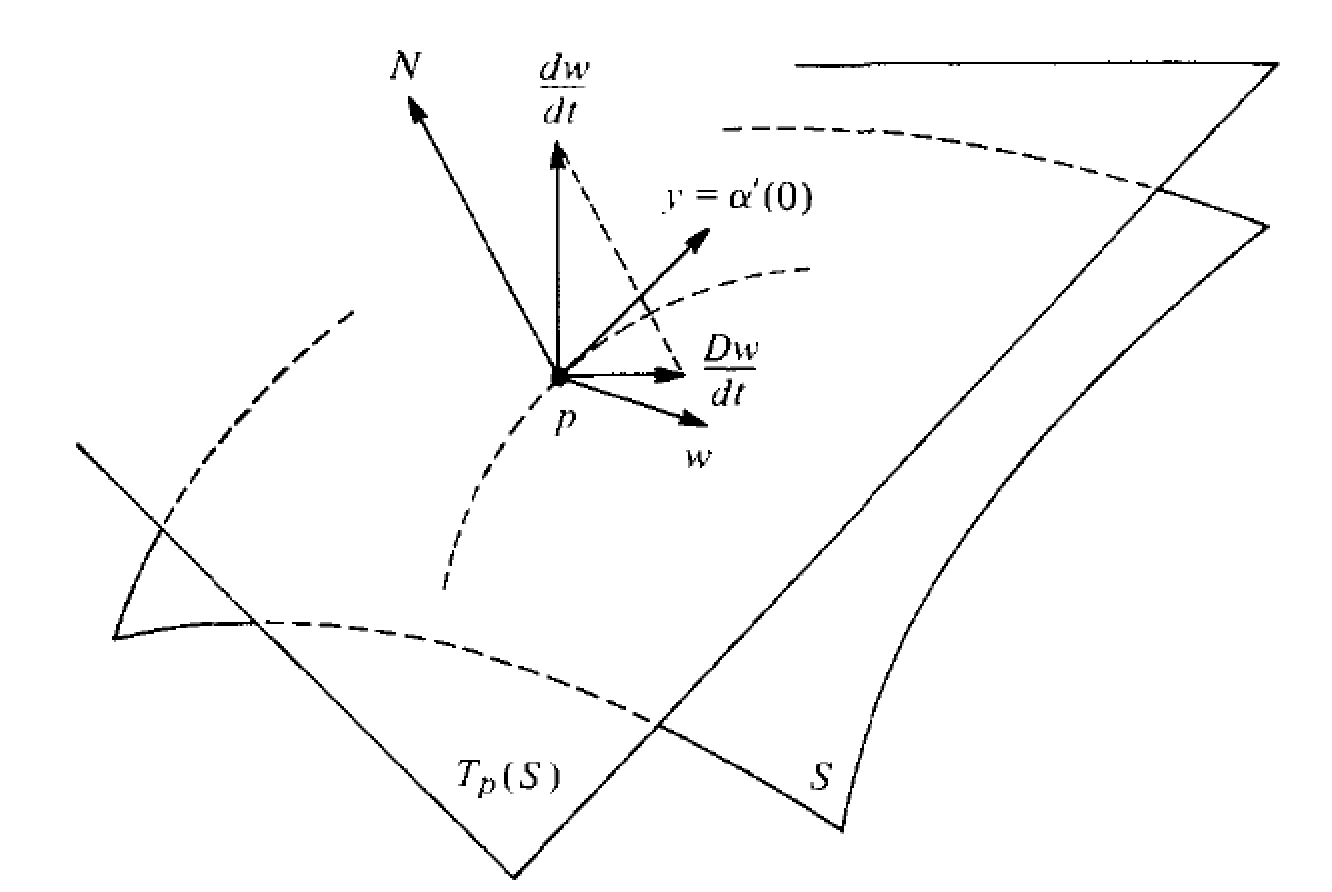
\includegraphics[scale = 0.43]{cov_deriv.png}}
\end{minipage}
\caption{\scriptsize
\textbf{The covariant derivative $\frac{D\mb{w}}{dt}$ at $p$ relative to vector $\mb{y}$, given by projection of Euclidean derivative $\frac{d\mb{w}}{dt}$ along the curve $\alpha$ with $\dot{\alpha} = \mb{y}$ onto the tangent plane of the surface. }}
\end{figure}

\item Intuitively $\frac{D\alpha'}{dt}$  is the \emph{acceleration} of the point $\alpha(t)$ "\emph{\textbf{as seen from the surface $\cS$}}."

\item Note that the concept of covariant derivative makes use of \textbf{normal vector} of $\cS$ and the \textbf{curve} $\alpha$ \textbf{tangent to} $\mb{y}$ at $p$. Its concern is the \underline{\emph{\textbf{rate of change}}} of the \emph{\textbf{vector field}} \underline{\emph{\textbf{along a curve}}}. 

\item The \emph{covariant derivative} only depends on the \emph{\textbf{intrinsic geometry of the surface}} and it does \emph{not} depend on the \emph{choice of the curve}. 

\item The concept of the \emph{covariant derivative} generalize the usual definition of the \emph{Euclidean derivative} as it take into account the \emph{\textbf{change of the basis vector}} of the \emph{tangent plane} \emph{along the curve on the surface} $\cS$ and only consider its \emph{\textbf{tangential projection}}. 

\item We can compare the difference when considering moving in plane vs. along a surface:
\begin{itemize}
\item For the differential of a vector field on \emph{Euclidean space}, the \textbf{basis} of the \emph{tangent plane} is defined \emph{\textbf{universally}} and they \emph{remain \textbf{unchanged} when \textbf{moving} on the plane}, whereas only the \emph{\textbf{component} of the differential} on each axis changes, i.e.
\begin{align*}
\frac{d\mb{w}}{dt} &= a'\mb{x}_{u} + b'\mb{x}_{v}.
\end{align*} 

\item However, when moving on the surface, given that these \emph{\textbf{components} of the differential} are unchanged, since the \textbf{axis} is \textbf{\emph{locally defined}}, the \textbf{basis} of the \emph{tangent plane} will \emph{\textbf{change}} when points moves, and it will cause the \emph{\textbf{change of the differential vector field}}, i.e. the differential of a vector field on the surface, 
\begin{align}
\frac{d\mb{w}}{dt} &= \set{a'\mb{x}_{u} + b'\mb{x}_{v}} + \set{a\paren{\mb{x}_{uu}u' + \mb{x}_{uv}v'} + b\paren{\mb{x}_{vu}u' + \mb{x}_{vv}v'}}, \label{eqn: change_of_vector_field}
\end{align} where $\mb{y} = \dot{\alpha}(0) = (u', v')$. 

It is noted that in ordinary Euclidean space, the derivative w.r.t. $t$ does not operate on the basis vector $\mb{c}=\mb{x}_{u}, \mb{d} = \mb{x}_{v}$ as they are \emph{\textbf{constant}} along \emph{\textbf{any curve in the space}}, thus in the first component $a', b'$ are the components of the acceleration vector along each axis. 

However, on the surface, the tangent space will '\emph{\textbf{rotate}}' as traversing along the curve. This second component accounts for that '\textbf{rotation}' effect. Note that it consists of second derivatives of curve so it is not necessarily on the tangent space. The covariant derivative is the projection of these terms into the tangent space. 
\end{itemize}

\item The \emph{covariant derivative} is given by observing that the \emph{\textbf{tangential component}} of the derivative $\frac{d\mb{w}}{dt}$ in \eqref{eqn: change_of_vector_field}. It consists of \textbf{two components}: 
\begin{enumerate}
\item The first one is the \emph{\textbf{tangential acceleration}} $a', b'$;
\item The second one is the \emph{\textbf{tangential component}} of \emph{\textbf{the second derivatives} of curve}, given by \emph{the Christoffel symbols}.
\end{enumerate}
For given $\mb{y}= (u', v') $ at $p$, 
\begin{align}
\frac{D\mb{w}}{dt} \equiv D_{\mb{y}}\mb{w} &= \paren{a' + \Gamma_{11}^{1}a\,u' + \Gamma_{12}^{1}a\,v' + \Gamma_{12}^{1}b\,u' +  \Gamma_{22}^{1}b\,v' } \mb{x}_{u} \nonumber\\
&+ \paren{b' + \Gamma_{11}^{2}a\,u' + \Gamma_{12}^{2}a\,v' + \Gamma_{12}^{2}b\,u' +  \Gamma_{22}^{2}b\,v' } \mb{x}_{v}    \label{eqn: cov_deriv_vec_field}
\end{align} 

From \eqref{eqn: cov_deriv_vec_field}, it is shown that the covariant derivative only depends on the vector $\mb{y} = (u', v')$ not on the curve $\alpha$. Also it is seen that it only depends on the \emph{Christoffel symbols} or the \emph{first fundamental form} (i.e. the \emph{instrinsic geometry of surface}). Thus \emph{\textbf{the covariant derivative is invariant under isometries}}.

For $\cS$ a plane, it is possible to find parameterization so that $E=G=1, F=0$, so $\Gamma_{i,j}^{k} = 0, \;\forall \,i,j,k=1,2$. Thus the covariant derivative become the usual Euclidean derivative. 

\item In general, the covariant derivative of $\mb{w} = \sum_{k}w_{k}\mb{x}_{k}$ relative to $\mb{y} = (y_{1}, y_{2})$ is given by 
\begin{align}
\frac{D\mb{w}}{dt} &= \mathcal{P}_{T_{p}S}\paren{\frac{d\mb{w}}{dt} }. \label{eqn: covariant_derivative_projection}\\
&= \sum_{k=1,2}\paren{w_{k}' + \sum_{i,j}\Gamma_{i,j}^{k} w_{i}\,y_{j} } \mb{x}_{k}.  \label{eqn: covariant_derivative_projection_christoffel}
\end{align}


\item \begin{definition}
A parameterized curve $\alpha: [0, l] \rightarrow \cS$ is the restriction to $[0,l]$ of a differentiable mapping of $(-\epsilon, l+\epsilon), \epsilon>0$ into $\cS$. If $\alpha(0) = 0, \alpha(l) = q$, we say that $\alpha$ \emph{\textbf{joins}} $p$ to $q$. $\alpha$ is regular if $\dot{\alpha}(t)\neq 0, \;t\in [0,l]$.
\end{definition}

\item \begin{definition}
Denote $I= [0,l]$. Let $\alpha: I\rightarrow \cS $ be a parameterized curve in $\cS$. A \emph{\textbf{vector field} $\mb{w}$ \textbf{along} $\alpha$} is a \emph{correspondence that assigns to each} $t\in I$ a vector 
\begin{align*}
\mb{w}(t) \in T_{\alpha(t)}\cS.
\end{align*}
The vector field is \emph{differentiable} at $t_{0}\in I$ if for some \emph{parameterization} $\mb{x}(u,v)$ in $\alpha(t_{0})$ the components $a(t), b(t)$ of $\mb{w}(t) = a\mb{x}_{u} + b\mb{x}_{v}$ are \emph{differentiable} functions of $t$ at $t_{0}$. $\mb{w}$ is \emph{differentiable} in $I$ if it is \emph{differentiable} for every $t\in I$.
\end{definition}

\item \begin{definition}
Let $\mb{w}$ be a differentiable vector field along $\alpha: I \rightarrow \cS$. The expression \eqref{eqn: cov_deriv_vec_field} of $\frac{D\mb{w}}{dt}(t)$, $t \in I$, is well defined and is called the \emph{\textbf{covariant derivative}} of $\mb{w}$ at $t$.
\end{definition}

\begin{figure}[thb]
\centering
\begin{minipage}{0.6\linewidth}
 \centerline{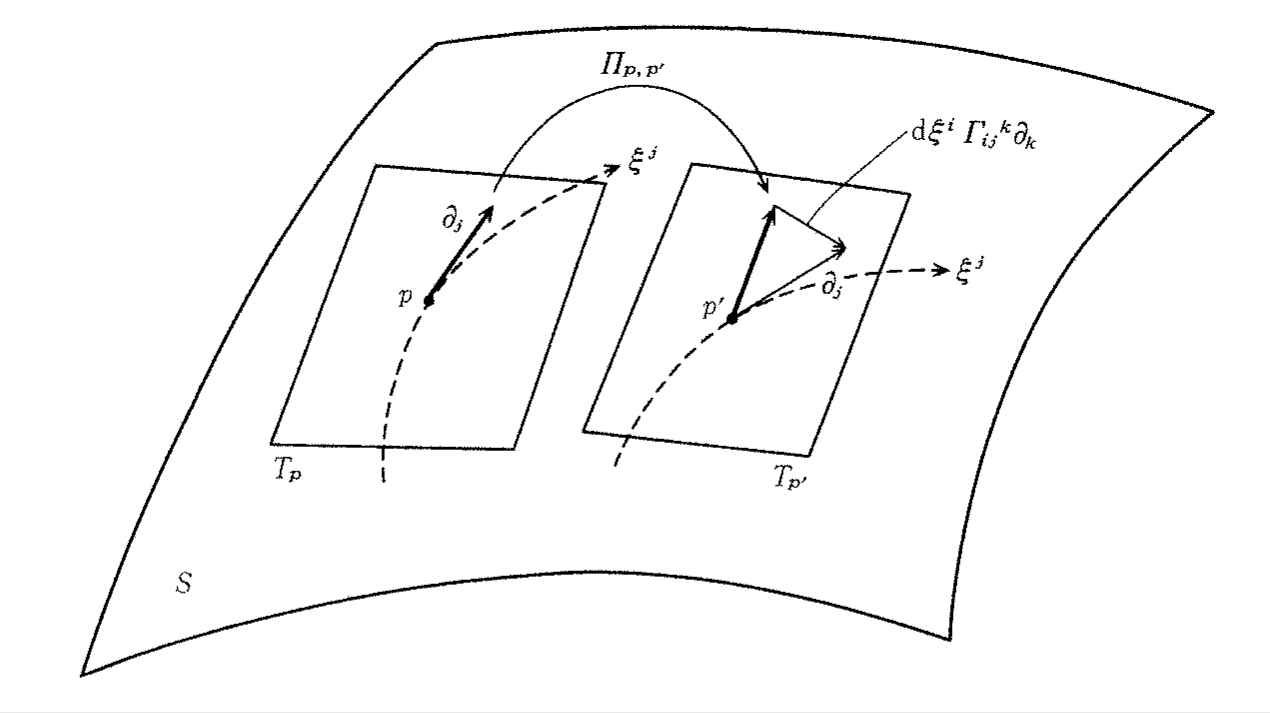
\includegraphics[scale = 0.43]{cov_deriv_comp.png}}
\end{minipage}
\caption{\scriptsize
\textbf{The covariant derivative $\nabla_{i}\mb{w}$ is seen as the usual partial derivative $\partial_{i}w^{k}$ combined with a linear compensation factor $w^{r}\Gamma_{r,i}^{k}$ that accounts for the change of the tangent plane of the surface. }}
\label{fig: cov_deriv_comp}
\end{figure}

\item The covariant derivative for basis vector field $\mb{w} =\mb{e}_{j}$ relative to vector $\mb{e}_{i}= \mb{x}_{\xi_{i}}$ can be expressed as 
\begin{align}
\nabla_{i}\mb{e}_{j}&= \mb{e}_{k}\Gamma_{i,j}^{k}\label{eqn: covariant_der_basis}
%\frac{D\mb{e}_{j}}{dt} &= \sum_{k}\mb{e}_{k}\Gamma_{i,j}^{k}
\end{align}
where the summation over $k$, who appears on both upper and lower indices, is omitted (called \emph{\textbf{Einstein's convention}} \citep{murray1993differential}).
Then for $\mb{w} = \sum_{k}w^{k}\,\mb{e}_{k}$ relative to vector $\mb{e}_{i}$ is given as 
\begin{align}
\nabla_{i}\mb{w}= \nabla_{i}\paren{w^{k}\mb{e}_{k} }&= \partial_{i}w^{k}\mb{e}_{k}+ w^{k}\mb{e}_{s}\Gamma_{k,i}^{s}\nonumber\\
&= \paren{\partial_{i}w^{k} + w^{r}\Gamma_{r,i}^{k}}\mb{e}_{k} =  \paren{\nabla_{i}\mb{w}^{k}}\mb{e}_{k}\nonumber\\
\text{or } \nabla_{i}\mb{w}^{k} &= \partial_{i}w^{k} + w^{r}\Gamma_{r,i}^{k} \label{eqn: cov_deriv_expr}
\end{align}
From the expression \eqref{eqn: cov_deriv_expr}, we see that the first term is the same as the gradient in Euclidean geometry, while the second term is related to the tangential projection of the rate of the change of the basis vector fields along the given basis direction. 



\item In general, the covariant derivative $\nabla_{\mb{y}}\mb{w}$ satisfies the following \textbf{properties}: for $\mb{w}, \mb{v}, \mb{y}, \mb{z}$ the vector field in $U\subset \cS$ and $f: U \rightarrow \bR$ is a differentiable function in $\cS$; $\nabla_{\mb{y}}\paren{f}$ is the directional derivative of $f$ in the direction of $\mb{y}$, $\lambda, \mu$ are real numbers, 
\begin{enumerate}
\item The \emph{\textbf{affine property}} for vector field 
 \begin{align}
\nabla_{\mb{y}}\paren{\lambda\mb{w}+ \mu\mb{v}} &= \lambda\nabla_{\mb{y}}\paren{\mb{w}}+ \mu\nabla_{\mb{y}}\paren{\mb{v}}; \nonumber\\
\nabla_{\lambda\mb{y}+ \mu\mb{z}}\paren{\mb{w}} &= \lambda\nabla_{\mb{y}}\paren{\mb{w}}+ \mu\nabla_{\mb{z}}\paren{\mb{w}} \label{eqn: connections_affine}
\end{align}
\item The \emph{\textbf{Leibniz rule}}
 \begin{align}
\nabla_{\mb{y}}\paren{f\mb{w}} &= \nabla_{\mb{y}}\paren{f}\mb{w}+ f\nabla_{\mb{y}}\paren{\mb{w}}; \nonumber\\
 \nabla_{f\mb{y}}\paren{\mb{v}} &=  f\nabla_{\mb{y}}\paren{\mb{v}}; \label{eqn: connections_leibniz}
\end{align}
\item The \emph{\textbf{metric-preserving property}}
\begin{align}
\nabla_{\mb{y}}\paren{\inn{\mb{w}}{\mb{v}}} &= \inn{\nabla_{\mb{y}}\paren{\mb{w}}}{\mb{v}} + \inn{\mb{w}}{\nabla_{\mb{y}}\paren{\mb{v}}}; \label{eqn: connections_metric}
\end{align}
\item The \emph{\textbf{symmetry property}}
\begin{align}
\nabla_{\mb{e}_{i}}\paren{\mb{e}_{j}} &= \nabla_{\mb{e}_{j}}\paren{\mb{e}_{i}}, \quad \mb{e}_{i} = \mb{x}_{\xi_{i}}\text{ for parameterization }\mb{x}(\xi_{1},\ldots, \xi_{m}).  \label{eqn: connections_symmetric}
\end{align}
The first two properties defines the \emph{\textbf{affine connection}} in $U\subset \cS$. The last two properties associate the connection with the \emph{\textbf{Riemannian metric}} and guarantee that the Christoffel symbols are symmetric w.r.t. lower indices. These four properties defines the \emph{\textbf{unique}} \underline{\emph{\textbf{connections}}} or \emph{covariant derivatives}, and \emph{parallel transport}, \emph{geodesic} on the surface. 
\end{enumerate}


\item We can use the property above to derive the covariant derivative of $\mb{w} = w_{k}\mb{e}_{k}$ with respect to $\mb{y} = y_{i}\mb{e}_{i}$
\begin{align*}
\nabla_{\mb{y}}\paren{\mb{w}} &= \nabla_{y_{i}\mb{e}_{i}}\paren{w_{k}\mb{e}_{k}}\\
&= y_{i}w_{k}\nabla_{\mb{e}_{i}}\paren{\mb{e}_{k}} +y_{i}\nabla_{\mb{e}_{i}}\paren{w_{k}}\mb{e}_{k} \\
&= \paren{y_{i}w_{k}\Gamma_{i,k}^{s}}\mb{e}_{s}+y_{i}\paren{\partial_{i}w_{k}}\mb{e}_{k}\\
&= \paren{y_{i}\paren{\partial_{i}w_{k}} + y_{i}\Gamma_{i,j}^{k}w_{j}  }\mb{e}_{k}
\end{align*}

\item In many books, the covariant derivative of vector field $\mb{w}$ relative to vector $\mb{y} = \dot{\alpha}(0)$ at $p$ as $\frac{D\mb{w}}{dt} \equiv D_{\mb{y}}\mb{w}$ is also denoted as $\nabla_{\mb{y}}\mb{w}$ \citep{do1992riemannian}. In particular, the operator $\nabla: C^{\infty}(\cS, T\cS) \times C^{\infty}(\cS, T\cS)\rightarrow C^{\infty}(\cS, T\cS)$ 
\begin{align*}
(\mb{Y}, \mb{W})\mapsto \nabla_{\mb{Y}}\mb{W}
\end{align*} is referred as an \underline{\emph{\textbf{affine connection}}} \citep{do1992riemannian, murray1993differential}, where $C^{\infty}(\cS, T\cS)$ is the space of differentiable vector fields on $\cS$, $T\cS = \set{(p,T_{p}\cS): p\in \cS}$ is the \emph{\textbf{tangent bundle}}. 

The \emph{affine connection} is a generalization of \emph{covariant derivative} since the direction along which the vector fields changes is also defined by a vector field. Thus it "\emph{connects}" two vector fields together.
\end{itemize}
\subsection{Parallel Transport}
\begin{itemize}
\item \begin{definition}
A \emph{vector field} $\mb{w}$ \emph{along a parameterized curve} $\alpha: I \rightarrow \cS$ is said to be \underline{\emph{\textbf{parallel}}} if $\frac{D\mb{w}}{dt} = 0$ for every $t\in I$.  
\end{definition} In other word, the vector fields $\mb{w}$ does not \emph{rotate} along the tangent direction of the curve $\alpha$.

\begin{figure}[tb]
\centering
\begin{minipage}{0.6\linewidth}
 \centerline{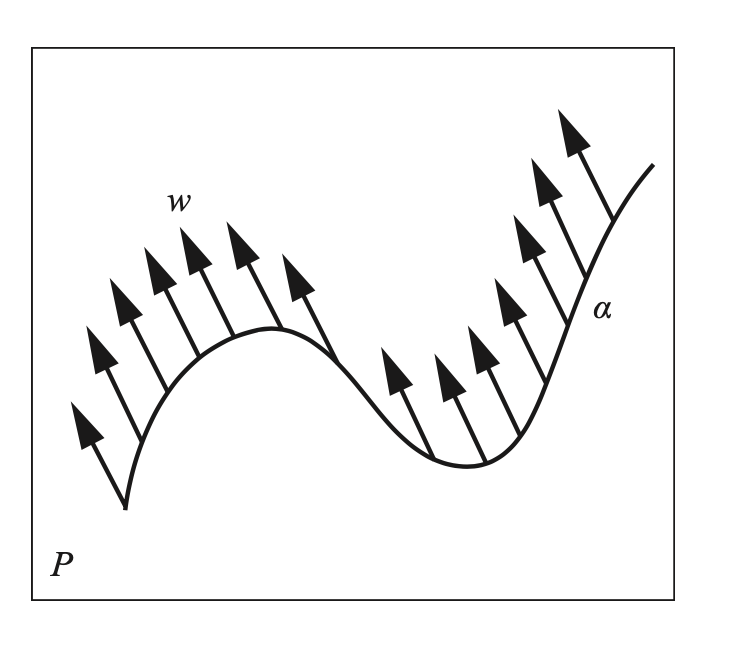
\includegraphics[scale = 0.43]{para_transp0.png}}
\end{minipage}
\caption{\scriptsize
\textbf{The vector field is parallel along the curve.}}
\label{fig: para_transp0}
\end{figure}

\item 
\begin{proposition}\label{prop: para_transp}
Let $\mb{w}, \mb{v}$ be parallel vector fields along $\alpha: I\rightarrow \cS$. Then $\inn{\mb{w}(t)}{\mb{v}(t)}$ is constant.  In particular, $\abs{\mb{w}(t)}$ and $\abs{\mb{v}(t)}$ are constant, and the \textbf{angle} between $\mb{w}, \text{and }\mb{v}$ is \textbf{constant}. 
\end{proposition}
\begin{proof}
Note that $\mb{w}$ is parallel along $\alpha$, which means that $\frac{D\mb{w}}{dt} =0$, or the differential of the vector field $\mb{w}':=\frac{d\mb{w}}{dt}$ is orthogonal to the tangent space $T_{\alpha(t)}\cS$, i.e.
\begin{align*}
\inn{\mb{w}'}{\mb{v}} &= 0;\quad \forall t\in I.
\end{align*}
Similarly, $\inn{\mb{w}}{\mb{v}'} = 0; \;\forall t\in I$. Therefore
\begin{align*}
\paren{\inn{\mb{w}(t)}{\mb{v}(t)}}' &= \inn{\mb{w}}{\mb{v}'}+ \inn{\mb{w}'}{\mb{v}} = 0,\;
\end{align*}
i.e. $\inn{\mb{w}(t)}{\mb{v}(t)} = c,\;\;\forall t\in I. $ \QEDA
\end{proof}

\item If the surface is \textbf{plane}, then the tangent vector field is \textbf{constant} along any curve; that is, the \emph{\textbf{angle}} with a fixed direction and the length of the vector are constant. 


\item  \begin{proposition}\label{prop: para_transp_curv}
Let $\alpha: I\rightarrow \cS$ be a parameterized curve in $\cS$ and let $\mb{w}_{0} \in T_{\alpha(t_{0})}S,\; t_{0}\in I$. There exists a \textbf{unique} \textbf{parallel} vector field $\mb{w}(t)$ along $\alpha(t)$, with $\mb{w}(t_{0}) = \mb{w}_{0}$. 
\end{proposition}
It shows that there exists a \emph{\textbf{unique}} vector field that is \emph{\textbf{parallel}} along any given regular curve and it only depends on one \emph{\textbf{initial vector}} in the \emph{tangent space}. 

\item \begin{proposition}\label{prop: geo_unique}
Given a point $p\in \cS$ and a vector $\mb{w}\in T_{p}(\cS), \mb{w}\neq 0$, there exists an $\epsilon>0$ and a unique parameterized geodesic $\gamma: (-\epsilon, \epsilon) \rightarrow \cS$ such that $\gamma(0)=p$ and $\dot{\gamma}(0) = \mb{w}$.
\end{proposition}

\item \begin{definition}
Let $\alpha: I \rightarrow \cS$ be a parameterized curve and $\mb{w}_{0}\in T_{\alpha(t_{0})}S$, $t_{0}\in I$. Let $\mb{w}$ be the \textbf{parallel vector field} along $\alpha$, with $\mb{w}(t_{0}) = \mb{w}_{0}.$ The vector $\mb{w}(t), t\in I$ is called the \underline{\emph{\textbf{parallel transport}}} of $\mb{w}(t_{0})= \mb{w}_{0}$ along $\alpha$ at point $t$.
\end{definition}
By using parallel transport, one can find the vector at \textbf{new point} in vector field from its value at old point \emph{along the curve}.  

\begin{figure}[tb]
\centering
\begin{minipage}{0.6\linewidth}
 \centerline{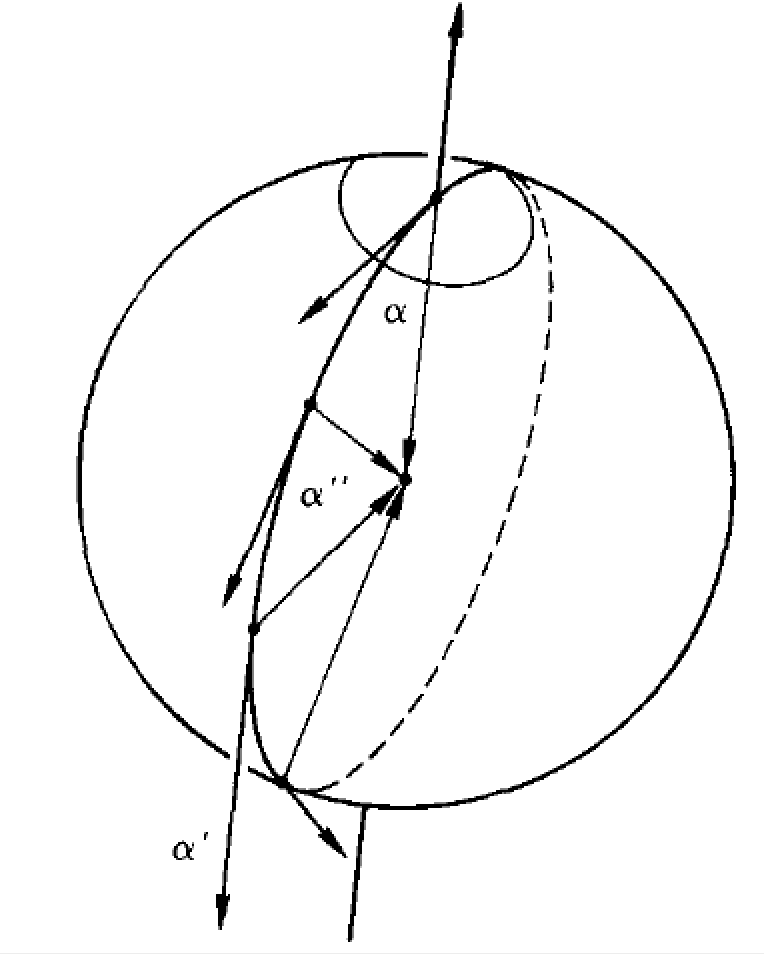
\includegraphics[scale = 0.43]{para_transp.png}}
\end{minipage}
\caption{\scriptsize
\textbf{For the sphere surface, the tangent vector field of any great circle is a parallel field on surface. Note that the differential of the tangent vector is normal to the surface, so its tangential component is zero.  }}
\end{figure}

\item Given that the curve $\alpha$ is regular, then the \emph{parallel transport} \textbf{\emph{does not depends on the parameterization}} of the curve. As for $\beta: J \rightarrow \cS$ another parameterization for the curve $\alpha(I)$, then 
\begin{align*}
\frac{D\mb{w}}{d\sigma} &= \frac{D\mb{w}}{dt}\frac{dt}{d\sigma}, \quad \forall t\in I, \sigma\in J.
\end{align*}
As $dt/d\sigma\neq 0$ then $\mb{w}(t)$ is parallel iff $\mb{w(\sigma)}$ is parallel. (Invariance to "change of parameterizations" is the result of invariance to isometry)

\item Some interesting properties of the parallel transport:
\begin{itemize}
\item \begin{proposition}
Define the linear mapping $P_{\alpha}: T_{p}(S) \rightarrow T_{q}(S)$ for $p,q\in \alpha$ that assign each $\mb{v}\in  T_{p}(S)$ its parallel transport at $q$ along $\alpha$. Then the map $P_{\alpha}$ is an \textbf{isometry}. 
\end{proposition}

In other word, the angle of the parallel transport of $\mb{w}$ along $\alpha$ to the tangent line of the curve $\dot{\alpha}$ is \textbf{constant}. 

\item If two surfaces are tangent along a curve $\alpha$ with a common vector $\mb{w}_{0} \in T_{\alpha(t)}S$ and $\mb{w}_{0} \in T_{\alpha(t)}\hat{S}$. Then the \emph{parallel transport} $\mb{w}(t)$ with initial vector $\mb{w}_{0}$ relative to $\cS$ is the same as that relative to $\hat{\cS}$, as it has the \emph{same covariant derivative along the curve}.
\end{itemize}

\item One can use these properties to find the parallel vector field along some curves. (Figure \ref{fig: example_parallel_transport})
\begin{figure}[htb]
\centering
\begin{minipage}{0.6\linewidth}
 \centerline{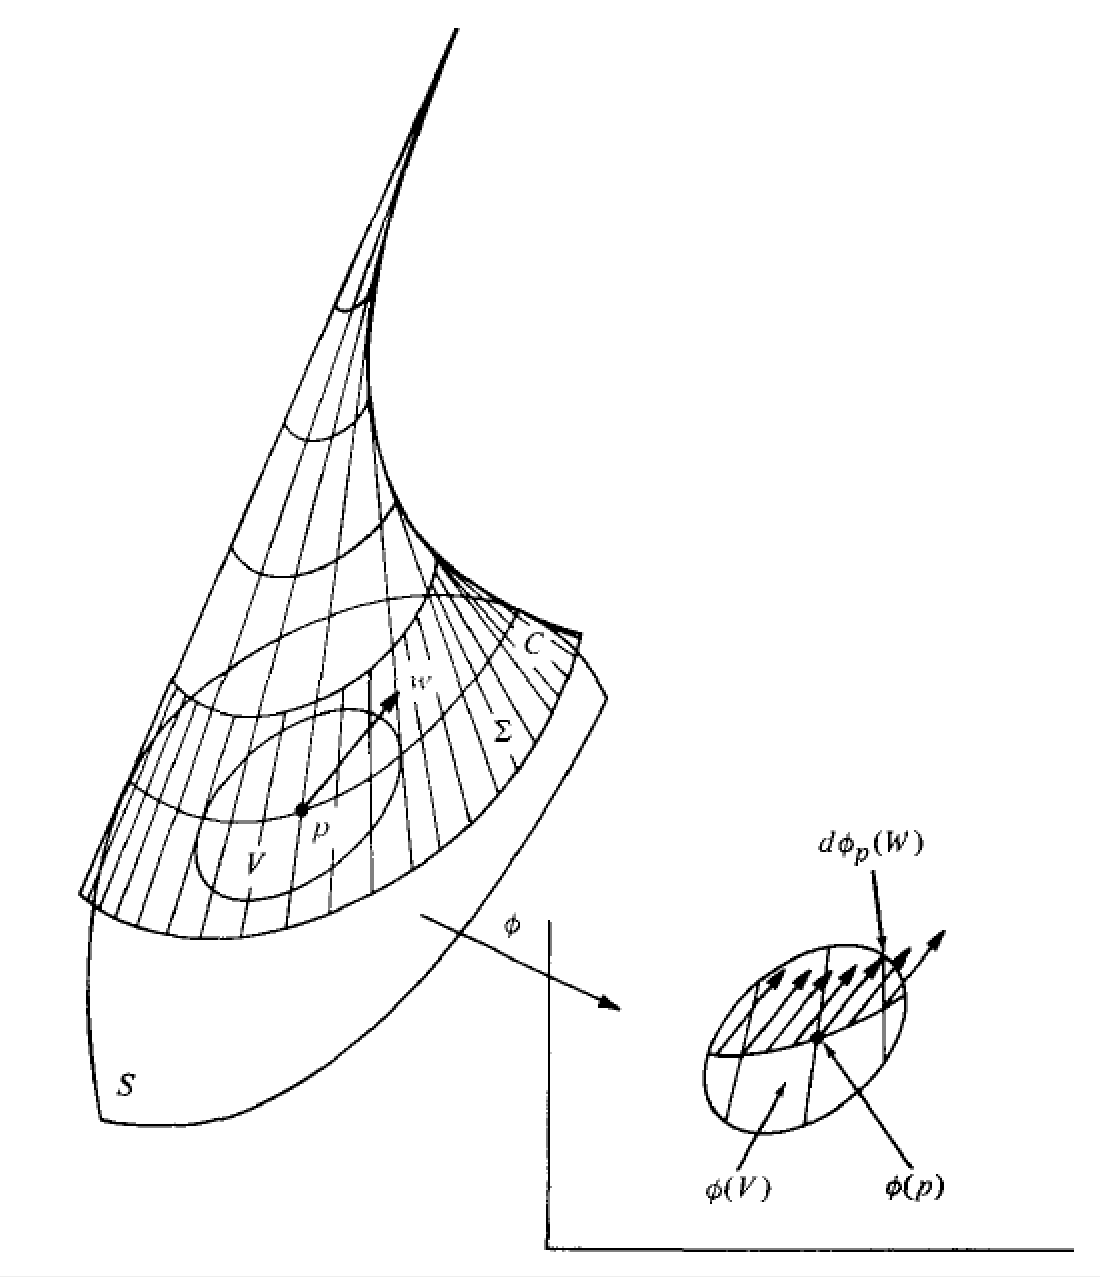
\includegraphics[scale = 0.43]{para_transp3.png}}
\end{minipage}
\caption{\scriptsize
\textbf{The parallel transport on the surface along $\cC$ is equal locally to those on the envelop of tangent plane of $\cC$.  By using the differential of an isometry $\varphi$, we can find a plane on which the parallel lines of the differential mapping $d\varphi(\mb{w})$ is a representation of the parallel transport.   }}
\label{fig: example_parallel_transport}
\end{figure}

Assume that a regular curve $\alpha$ joins two points $p,q$ on $\cS$ and it is nowhere tangent to the asymptotic directions. Consider the envelop of the family of tangent planes of $\cS$ along $\alpha$. In a neighborhood of $\alpha$, this envelop is a regular surface $\Sigma$ which is \emph{tangent to} $\cS$ along $\alpha$. Then we see that the parallel transport of $\mb{w}$ along $\alpha$ is \textbf{the same} no matter which surface $\cS$ or $\Sigma$ is concerned. 

It can be shown that the \emph{Gaussian curvature} of $\Sigma$ is zero, i.e. it is \emph{locally isometric} to a plane. Hence, we can find a neighborhood $V\subset \Sigma$ of $p$ into a plane $P$ by an isometry $\varphi: V\rightarrow P$. To obtain the parallel transport of $\mb{w}$ along $V\cap \alpha$, we can take the usual parallel transport in the plane of $d\varphi_{p}(\mb{w})$ along $\varphi\circ  \alpha$. Then pull it back to $\Sigma$ by $d\varphi$.

This shows a geometric interpretation of the parallel transport.

\item A \textbf{straight line} at the \textbf{plane} is seen as \emph{\textbf{parallel transport}} of the tangent vector $\dot{\alpha}$ along the curve of $\alpha$, i.e. the only curve that maintain the direction and length of its tangent line unchanged is the straight line on the plane. 
\end{itemize}

\subsection{Geodesic}
\begin{itemize}
\item \begin{definition}
A nonconstant, parameterized curve $\gamma: I \rightarrow \cS$ is said to be \underline{\emph{\textbf{geodesic}}} at $t\in I$ if the \textbf{field of its \emph{tangent vectors}} $\dot{\gamma}(t)$ is \textbf{\emph{parallel}} along $\gamma$ at $t$; that is, 
\begin{align*}
\frac{D\dot{\gamma}(t)}{dt} = 0;
\end{align*}
$\gamma$ is a \emph{\textbf{parameterized geodesic}} if it is \emph{geodesic} for all $t\in I$.
\end{definition} It is seen that $\abs{\dot{\gamma}(t)} = c\neq 0$ and the geodesic can be reparameterized by its arc length $s$.


\item \begin{definition}
A \emph{regular} \emph{connected} curve $\cC$ in $\cS$ is said to be a \emph{\textbf{geodesic}} if, for every $p\in \cC$, the parameterization $\alpha(s)$ of a coordinate neighborhood of $p$ by arc length $s$ is a \emph{\textbf{parameterized geodesic}}; that is $\dot{\alpha}(s)$ is a \emph{\textbf{parallel vector field}} along $\alpha(s)$.
\end{definition}

\begin{figure}[htb]
\centering
\begin{minipage}{0.6\linewidth}
 \centerline{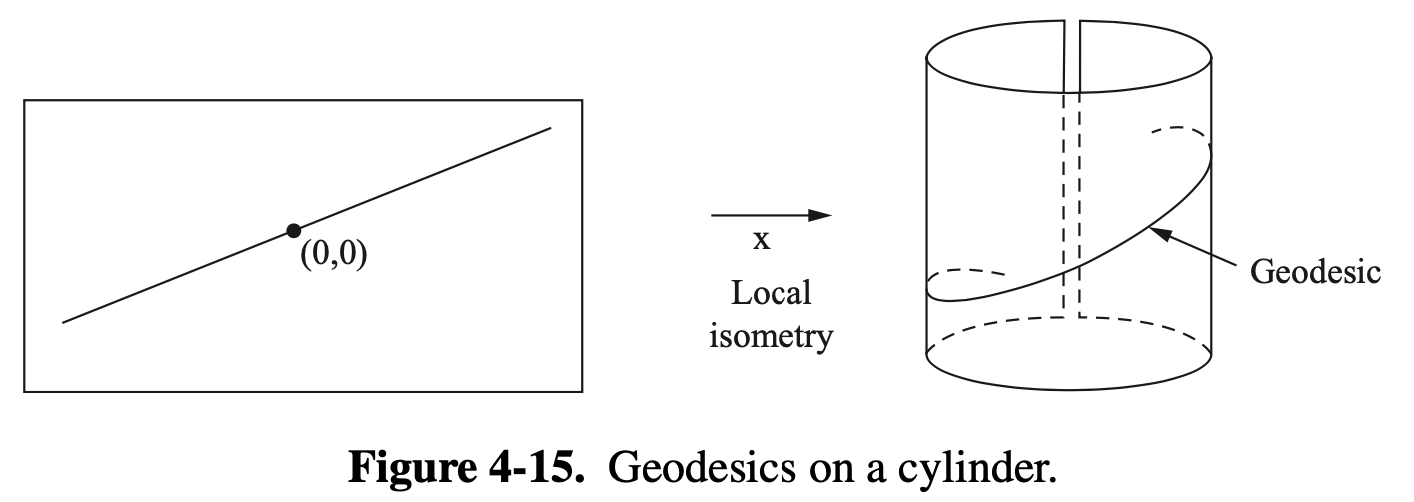
\includegraphics[scale = 0.6]{geodesic_cyliner.png}}
\end{minipage}
\caption{\scriptsize
\textbf{The geodesic on a cylinder.}}
\label{fig: geodesic_cyliner}
\end{figure}


\item Assume the curve $\alpha(t)$ is a motion on $\cS$ with \emph{\textbf{unit velocity}} $\dot{\alpha}(t)$. The trajectory of $\alpha(t)$ at a given interval $I$ is a geodesic iff the \emph{\textbf{acceleration vector}} $\dot{\alpha}'(t) = k\mb{n}$ is \emph{\textbf{normal} to the tangent plane of the surface}, or the tangential acceleration is zero. In other word, a regular curve $\cS \subset \cS$ is a geodesic iff its principal normal (, i.e. the line that contains $\mb{n}$ and passes through $\cC$) at each point $p\in \cC$ is parallel to the normal to $\cS$ at $p$.
  
\item \begin{definition}
Let $\mb{w}$ be a differentiable vector field of \emph{\textbf{unit vectors}} along a parameterized curve $\alpha: I \rightarrow \cS$ on an \emph{\textbf{oriented surface}} $\cS$. Since $\mb{w}(t), t\in I$ is a unit vector field, $d\mb{w}(t)/dt$ is \textbf{normal to} $\mb{w}(t)$, and therefore, 
\begin{align*}
\frac{D\mb{w}}{dt} &= \lambda\,\paren{\mb{N} \wedge \mb{w}(t)},
\end{align*} 
where $\lambda = \lambda(t)$ denoted as $\brac{D\mb{w}/dt}$, is called \underline{\emph{\textbf{the algebraic value}}} of the \emph{covariant derivative} of $\mb{w}$ at $p$.
\end{definition}

Note that $\lambda = \brac{D\mb{w}/dt} = \inn{d\mb{w}(t)/dt}{\mb{N} \wedge \mb{w}}$ and its sign depends on the \emph{\textbf{orientation}} of the surface. 

\item The concept of \emph{parallel transport} and \emph{geodesic} does \textbf{not} depend on the \emph{\textbf{orientation}} of the surface. But the \emph{\textbf{geodesic curvature}} \emph{changes its sign} with the \emph{change of orientation} of the surface.

\item \begin{definition}
Let $\cC$ be an \emph{\textbf{oriented}} \emph{regular curve} contained on an \emph{oriented surface} $\cS$, and let $\alpha(s)$ be a parameterization of $\cC$ in a neighborhood of $p\in \cS$, by the arc length $s$. The \emph{\textbf{algebraic value}} of the \emph{covariant derivative} $\brac{D\dot{\alpha}(s)/ds} = k_{g}$ at $p$ is called the \underline{\emph{\textbf{geodesic curvature}}} of $\cC$ at $p$. 
\end{definition}
Any oriented regular curve can have geodesic curvature. The regular \textbf{geodesic curve} is characterized as the regular curve whose \emph{\textbf{geodesic curvature is zero}}.  

\begin{figure}[tbh]
\centering
\begin{minipage}{0.6\linewidth}
 \centerline{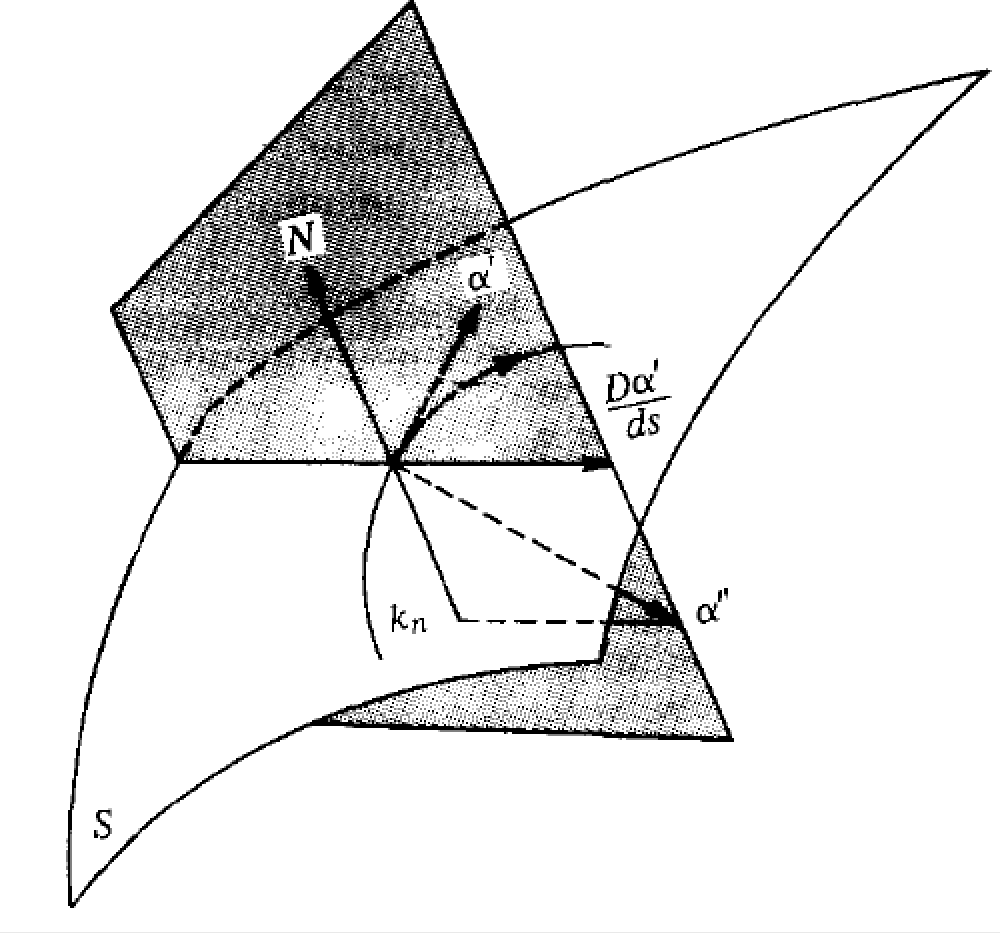
\includegraphics[scale = 0.43]{geo_curv.png}}
\end{minipage}
\caption{\scriptsize
\textbf{The geodesic curvature given by projecting $\dot{\alpha}'$ to the tangent plane. Its projection on the normal plane is the normal curvature.   }}
\label{fig: geo_curv}
\end{figure}


\item The absolute value of the geodesic curvature $k_{g}$ of $\cC$ at $p$ is \emph{tangential component} of the vector $\dot{\alpha}'(s)= k\mb{n}$, where $k$ is the curvature of $\cC$ and $\mb{n}$ is the normal vector of the curve $\cC$. Note that the absolute value of its \emph{normal component} is the absolute value of the \textbf{\emph{normal curvature}} $k_{n}$. So
\begin{align*}
k^{2} = k_{g}^{2} + k_{n}^{2}.
\end{align*} The absolute value of the \textbf{\emph{geodesic curvature}} is the same if two surfaces are \emph{\textbf{tangent} along the curve}. See Figure \ref{fig: geo_curv}.

\item For unit vector field $\mb{w}$ parallel along the curve $\alpha$, 
\begin{align*}
\frac{D\mb{w}}{dt} &= 0 = k_{g}\paren{\mb{N} \wedge \mb{w}(t)}.
\end{align*} 
So $k_{g}=0= \frac{d\phi}{ds}$. It means that the \textbf{angle} that the \emph{\textbf{tangent}} to the curve makes with a \emph{\textbf{parallel}} direction along the curve is constant. 

If the curve $\alpha = \gamma$ is the geodesic, then the angle of the \emph{\textbf{velocity}} of the geodesic makes with the \emph{parallel direction} of the field is \textbf{unchanged} during the movement. 
\begin{figure}[htb]
\centering
\begin{minipage}{0.6\linewidth}
 \centerline{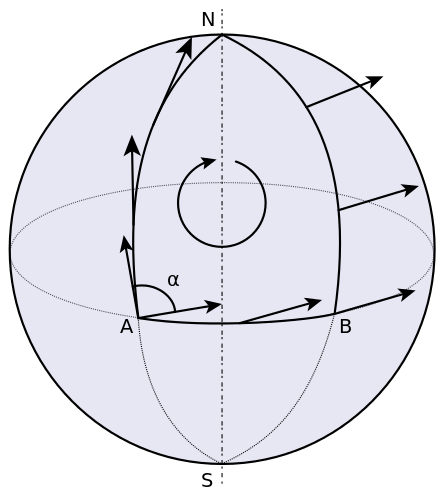
\includegraphics[scale = 0.3]{Parallel_Transport.png}}
\end{minipage}
\caption{\scriptsize
\textbf{The unit vector field that is parallel along a geodesic curve then the angle from the velocity of the geodesic to the parallel direction of the field is constant along the trajectory.  in this plot, the parallel transport of a vector around a closed loop (from $A$ to $N$ to $B$ and back to $A$) on the sphere. The angle by which it twists, $\alpha$, is proportional to the area inside the loop. }} 
\end{figure}

\item \begin{lemma}\label{lem: diff_angle}
Let $a,b$ be differentiable functions in $I$ with $a^{2}+ b^{2} = 1$ and $\phi_{0}$ be such that $a_{0} = \cos \phi_{0}$ and $b_{0} = \sin \phi_{0}$. Then the differentiable function 
\begin{align*}
\phi &= \phi_{0} + \int_{t_{0}}^{t}\paren{ab' - a'b}dt
\end{align*}
is such that $\cos \phi = a(t)$ and $\sin \phi = b(t), t\in I,$ and $\phi\paren{t_{0}} = \phi_{0}$.
\end{lemma}

\item \begin{lemma} \label{lem: cov_deriv_angle}
Let $\mb{v,w}$ be two differentiable vector fields along the curve $\alpha: I \rightarrow \cS$, with $\abs{\mb{w}(t)} = \abs{\mb{v}(t)} = 1$, $t\in I$. Then 
\begin{align*}
\brac{\frac{D\mb{w}}{dt}} - \brac{\frac{D\mb{v}}{dt}} &= \frac{d\phi}{dt},
\end{align*}
where $\phi$ is one of the \textbf{differentiable} \textbf{determination} of the \textbf{angle} from $\mb{v}$ to $\mb{w}$, as given in Lemma \ref{lem: diff_angle}
\end{lemma}
\begin{proof}
We introduce the vectors $\hat{\mb{v}} = \mb{N}\wedge \mb{v}$ and $\hat{\mb{w}} = \mb{N}\wedge \mb{w}$. Then 
\begin{align}
\mb{w} &= (\cos\phi)\,\mb{v} + (\sin(\phi))\,\hat{\mb{v}}, \label{eqn: cov_deriv_angle_1}\\
\hat{\mb{w}} =  \mb{N}\wedge \mb{w} &= (\cos\phi)\,\mb{N}\wedge\mb{v} + (\sin\phi)\,\mb{N}\wedge \hat{\mb{v}} \nonumber\\
&= (\cos\phi)\,\hat{\mb{v}} - (\sin\phi)\,\mb{v}. \label{eqn: cov_deriv_angle_2}
\end{align}
By differentiating \eqref{eqn: cov_deriv_angle_1} w.r.t. $t$, we obtain
\begin{align*}
\mb{w}' &= -(\sin\phi)\phi'\,\mb{v} + (\cos\phi)\,\mb{v}' + (\cos\phi)\phi'\,\hat{\mb{v}} + (\sin\phi)\,\hat{\mb{v}}'
\end{align*}
and we take inner product with $\hat{\mb{w}}$ via  \eqref{eqn: cov_deriv_angle_2} and $\inn{\mb{v}'}{\mb{v}} = \inn{\hat{\mb{v}}}{\mb{v}} =\inn{\hat{\mb{v}}'}{\hat{\mb{v}} } =  0$ as
\begin{align*}
\inn{\mb{w}' }{\hat{\mb{w}}}&= \inn{-(\sin\phi)\phi'\,\mb{v} + (\cos\phi)\,\mb{v}' + (\cos\phi)\phi\,\hat{\mb{v}} + (\sin\phi)\,\hat{\mb{v}}'}{ (\cos\phi)\,\hat{\mb{v}} - (\sin\phi)\,\mb{v}}\\
&= (\sin\phi)^{2}\phi' - \cos\phi\,\sin\phi \inn{\mb{v}'}{\mb{v}} -\cos\phi\,\sin\phi\,\phi'\,\inn{\hat{\mb{v}}}{\mb{v}}
- (\sin\phi)^{2}\inn{\hat{\mb{v}}'}{\mb{v}} \\
&-\cos\phi\,\sin\phi\,\phi'\inn{\hat{\mb{v}}}{\mb{v}} +  (\cos\phi)^{2}\inn{\hat{\mb{v}}}{\mb{v}'} + (\cos\phi)^{2}\phi'
+ \cos\phi\,\sin\phi \inn{\hat{\mb{v}}'}{\hat{\mb{v}} }\\
&=  (\sin\phi)^{2}\phi' - (\sin\phi)^{2}\inn{\hat{\mb{v}}'}{\mb{v}} +  (\cos\phi)^{2}\inn{\hat{\mb{v}}}{\mb{v}'} + (\cos\phi)^{2}\phi'\\
& = \phi'- (\sin\phi)^{2}\inn{\hat{\mb{v}}'}{\mb{v}} +  (\cos\phi)^{2}\inn{\mb{v}'}{\hat{\mb{v}}}.
\end{align*}
Note that $\inn{\hat{\mb{v}}}{\mb{v}}  = 0$ so $\inn{\hat{\mb{v}}}{\mb{v}'}  = - \inn{\hat{\mb{v}}'}{\mb{v}}  $. So the above expression is
\begin{align*}
\inn{\mb{w}' }{\hat{\mb{w}}}&= \phi' + \inn{\mb{v}'}{\hat{\mb{v}}}
\end{align*}

It then follows that 
\begin{align*}
\brac{\frac{D\mb{w}}{dt}} &= \inn{\mb{w}' }{\hat{\mb{w}}} =  \phi' + \inn{\mb{v}'}{\hat{\mb{v}}} = \frac{d\phi}{dt} + \brac{\frac{D\mb{v}}{dt}},
\end{align*}
since 
\begin{align*}
 \inn{\mb{w}' }{\hat{\mb{w}}}  &= \inn{\frac{d\mb{w}}{dt}}{\mb{N}\wedge\mb{w}} = \brac{\frac{D\mb{w}}{dt}}\norm{\mb{N}\wedge\mb{w}}{}^{2} =  \brac{\frac{D\mb{w}}{dt}}.
\end{align*}\QEDA
\end{proof}


\item An immediate consequence of the above lemma is the following observation. 

The \emph{\textbf{geodesic curvature}} is the \emph{\textbf{rate of change} of the \textbf{angle} that the \textbf{tangent} to the \textbf{curve} makes with a \textbf{parallel direction} along the curve}. That is, define $\mb{w}, \mb{v}$ be two vector field with unit length $\abs{\mb{w}} = \abs{\mb{v}} = 1$ and a differentiable map $\phi: I \rightarrow \bR$ to be the angle from $\mb{v}(t)$ to $\mb{w}(t)$ in the orientation of the surface. Then 
\begin{align*}
k_{g}(s) &= \brac{\frac{D\dot{\alpha}(s)}{ds}} = \frac{d\phi}{ds}.
\end{align*}
For a \textbf{plane}, as the \emph{parallel direction} is \textbf{constant}, the \textbf{geodesic curvature} becomes the usual \textbf{curvature}.

\item $k_g = 0$ can be seen as an generalization of straight line in plane towards surface, where the velocity of motion does not change direction along the line.

\item \begin{proposition}\label{prop: alg_value_angle} (\textbf{The algebraic value in terms of first fundamental form})\\
Let $\mb{x}(u,v)$ be an \textbf{orthogonal parameterization} ($F=0$) of a neighborhood of an oriented surface $\cS$, and $\mb{w}(t)$ be a differentiable vector field of \textbf{unit vectors} along the curve $\mb{x}(u(t), v(t))$. Then 
\begin{align}
\brac{\frac{D\mb{w}}{dt}} &= \frac{1}{2\sqrt{EG}}\set{G_{u}\frac{dv}{dt} - E_{v}\frac{du}{dt} } +  \frac{d\phi}{dt}, \label{eqn: algebraic_value_first_fundamental_form}
\end{align}
where $\phi(t)$ is the angle from $\mb{x}_{u}$ to $\mb{w}(t)$ in the given orientation. 
\end{proposition}
\begin{proof}
Let $\mb{e}_{1} = \mb{x}_{u}/\sqrt{E}$ and $\mb{e}_{2} = \mb{x}_{v}/\sqrt{G}$ be the unit vectors tangent to the coordinate curves. Observe that $\mb{e}_{1} \wedge \mb{e}_{2} = \mb{N}$, where $\mb{N}$ is the normal vector in the given orientation of $\cS$. By using Lemma \eqref{lem: cov_deriv_angle}, we write
\begin{align*}
\brac{\frac{D\mb{w}}{dt}} &=  \frac{d\phi}{dt} + \brac{\frac{D\mb{e}_{1}}{dt}}, 
\end{align*}
where $\mb{e}_{1}(t) = \mb{e}_{1}(u(t), v(t))$ is the field of $\mb{e}_{1}$ restricted to the curve $\mb{x}(u(t), v(t))$. Now 
\begin{align*}
\brac{\frac{D\mb{e}_{1}}{dt}} = \inn{\frac{d\mb{e}_{1}}{dt}}{ \mb{N}\wedge \mb{e}_{1} }
&=  \inn{\frac{d\mb{e}_{1}}{dt}}{\mb{e}_{2} }\\
&= \frac{du}{dt}\inn{\paren{\mb{e}_{1}}_{u}}{\mb{e}_{2}} + \frac{dv}{dt}\inn{\paren{\mb{e}_{1}}_{v}}{\mb{e}_{2}}.
\end{align*}

On the other hand, given that $F=0$, 
\begin{align*}
\inn{\mb{x}_{uu}}{\mb{x}_{v}} &= -\frac{1}{2}E_{v}
\end{align*}
and therefore,
\begin{align*}
\inn{\paren{\mb{e}_{1}}_{u}}{\mb{e}_{2}} &= \inn{\paren{\frac{\mb{x}_{u}}{\sqrt{E}}}_{u}}{\frac{\mb{x}_{v}}{\sqrt{G}}}
= -\frac{E_{v}}{2\sqrt{EG}}.
\end{align*}
Similarly, 
\begin{align*}
\inn{\paren{\mb{e}_{1}}_{v}}{\mb{e}_{2}} &= \inn{\paren{\frac{\mb{x}_{u}}{\sqrt{E}}}_{v}}{\frac{\mb{x}_{v}}{\sqrt{G}}}
= \frac{G_{u}}{2\sqrt{EG}}.
\end{align*}
Then substituting these equations into the expression of $\brac{\frac{D\mb{w}}{dt}} $, we obtain
\begin{align*}
\brac{\frac{D\mb{w}}{dt}} &=  \frac{1}{2\sqrt{EG}} \set{G_{u}\frac{dv}{dt}  -E_{v}\frac{du}{dt} } +\frac{d\phi}{dt} 
\end{align*} \QEDA
\end{proof}

From this proposition, we see that the \emph{\textbf{algebraic value}}, like covariant derivative and geodesic, is also function of first fundamental form, thus it only depends on the \emph{\textbf{intrinsic  geometry of surface}}.


\item \begin{proposition}\label{prop: liouville_formula}
(\textbf{Decomposition of geodesic curvature})[\textbf{Liouville}] \citep{do1976differential}.\\
Let $\alpha(s)$ be a parameterization by arc length of a neighborhood of a point $p\in \cS$ of a regular oriented curve $\cC$ on an oriented surface $\cS$.  Let $\mb{x}(u,v)$ be an \textbf{orthogonal parameterization} ($F=0$) of $\cS$ at $p$ and $\phi(s)$ be the \textbf{angle} that $\mb{x}_{u}$ makes with $\dot{\alpha}(s)$ in the given orientation. Then 
\begin{align}
k_{g} &= (k_{g})_{1}\cos\phi + (k_{g})_{2}\sin\phi + \frac{d\phi}{ds}  \label{eqn: geodesic_curvature_liouville}
\end{align}
where $(k_{g})_{1}$ and $ (k_{g})_{2}$ are geodesic curvature of the coordinate curves $v=const.$ and $u=const.$ respectively. 
\end{proposition}
\begin{proof}
By setting $\mb{w} = \dot{\alpha}(s)$ in Proposition \eqref{prop: alg_value_angle}, we obtain
\begin{align*}
\brac{\frac{D\dot{\alpha}}{ds}} = k_{g}&=  \frac{1}{2\sqrt{EG}} \set{G_{u}\frac{dv}{ds}  -E_{v}\frac{du}{ds} } +\frac{d\phi}{ds} 
\end{align*}

Note that along the coordinate curve $v= const. $, $\frac{dv}{ds} = 0,\;\frac{du}{ds} = \frac{1}{\sqrt{E}}$. Also for $u= const. $, $\frac{du}{ds} = 0, \frac{dv}{ds} = \frac{1}{\sqrt{G}}$. Therefore,
\begin{align*}
 (k_{g})_{1} =  -\frac{E_{v}}{2E\sqrt{G}} &&  (k_{g})_{2} =  \frac{G_{u}}{2G\sqrt{E}} .
\end{align*}

By introducing these relations in the above formula, we obtain that
\begin{align*}
 k_{g}&= \set{(k_{g})_{1}\sqrt{E}\frac{du}{ds} + (k_{g})_{2} \sqrt{G} \frac{dv}{ds}} +\frac{d\phi}{ds}.
\end{align*}

Since 
\begin{align*}
\sqrt{E}\frac{du}{ds} & = \inn{\mb{x}_{u}\frac{du}{ds}}{\frac{\mb{x}_{u}}{\sqrt{E}}} \\
&= \inn{\mb{x}_{u}\frac{du}{ds}+ \mb{x}_{v}\frac{dv}{ds}}{\frac{\mb{x}_{u}}{\sqrt{E}}}\\
&= \inn{\dot{\alpha}(s)}{\frac{\mb{x}_{u}}{\sqrt{E}}} = \cos\phi
\end{align*}
and $\sqrt{G} \frac{dv}{ds} =  \inn{\dot{\alpha}(s)}{\frac{\mb{x}_{v}}{\sqrt{G}}} = \sin\phi$, we finally reach 
\begin{align*}
k_{g} &= (k_{g})_{1}\cos\phi + (k_{g})_{2}\sin\phi + \frac{d\phi}{ds}.
\end{align*}
This formula is called \emph{Liouville formula}. \QEDA 
\end{proof}

\item In the geodesic polar system $(\rho, \theta)$, Then the coefficients $E\equiv E(\rho, \theta)$, $F\equiv F(\rho, \theta)$ and $G\equiv G(\rho, \theta)$ of the first fundamental form satisfies the conditions
\begin{align}
E = 1, && F=0, && \sqrt{G}=\rho &\Rightarrow& \lim_{\rho \rightarrow 0}G = 0, && \lim_{\rho\rightarrow 0}(\sqrt{G})_{\rho} = 1. \label{eqn: Gauss_lemma}
\end{align}
\end{itemize}

\subsection{The equations of a geodesic}
\begin{itemize}
\item The \emph{\textbf{geodesic}} is defined as the parameterized curve $\gamma: I \rightarrow \cS$ whose tangent vector field $\dot{\gamma}(s)$ is \emph{parallel} along the curve $\gamma(s)$.  Specifically, let $\mb{x}(u,v)$ be a parameterization of the surface in the neighborhood $V$ of $\gamma(t_{0}), t_{0}\in I$. There exists an open interval $J \subset I$, $\gamma(J) \subset V$. Let $\mb{x}(u(t), v(t)), t\in J$ be the expression of $\gamma: J  \rightarrow \cS$ in the parameterization of $\cS$. 

Then the tangent vector field $\dot{\gamma}(t), t\in J$ is given as 
\begin{align*}
\dot{\gamma}(t) &= u'(t)\mb{x}_{u} + v'(t)\mb{x}_{v}.
\end{align*}
So by substituting \eqref{eqn: cov_deriv_vec_field} with $a= u', b= v'$,  the equation  $\frac{D\dot{\gamma}(t)}{dt} = 0$ can be represented as
\begin{align*}
\frac{D\dot{\gamma}}{dt} &= \paren{u'' + \Gamma_{11}^{1}\paren{u'}^{2} + \Gamma_{12}^{1}u'\,v' + \Gamma_{12}^{1}v'\,u' +  \Gamma_{22}^{1}\paren{v'}^{2} } \mb{x}_{u} \nonumber\\
&+ \paren{v'' + \Gamma_{11}^{2}\paren{u'}^{2}+ \Gamma_{12}^{2}u'\,v'+ \Gamma_{12}^{2}v'\,u'+  \Gamma_{22}^{2}\paren{v'}^{2} } \mb{x}_{v} = 0
\end{align*}
or 
\begin{align}
u'' + \Gamma_{11}^{1}\paren{u'}^{2} + 2\Gamma_{12}^{1}u'\,v' +  \Gamma_{22}^{1}\paren{v'}^{2} &=0\nonumber\\
v'' + \Gamma_{11}^{2}\paren{u'}^{2}+ 2\Gamma_{12}^{2}u'\,v'+  \Gamma_{22}^{2}\paren{v'}^{2}&=0\label{eqn: geo_diff_eqn}
\end{align}
It can be generalized to \emph{high dimensional space} as the \textbf{parameterization} $\mb{x}(\xi_{1},\ldots, \xi_{n})$
\begin{align}
\frac{d^{2} \xi^{k}}{dt^{2}} + \sum_{i,j \in \set{1,\ldots,n}^{2}}\Gamma_{i,j}^{k}\frac{d\xi^{i}}{dt}\frac{d\xi^{j}}{dt} = 0, \quad k=1,\ldots, n.\label{eqn: geo_diff_eqn_high}
\end{align} 
Note that $\Gamma_{i,j}^{k},\; i,j,k=1,\ldots,n$ are functions of intrinsic coordinate functions $(\xi_{1}(t),\ldots, \xi_{n}(t)).$ 

In other words, $\gamma$ is the \emph{geodesic} \emph{\textbf{if and only if}} the differential equations \eqref{eqn: geo_diff_eqn} is satisfied for every interval $J \subset I$ such that $\gamma(J)$ is contained in a coordinate neighborhood. 

The system \eqref{eqn: geo_diff_eqn} (or \eqref{eqn: geo_diff_eqn_high}) is known as \underline{\emph{\textbf{the differential equations of the geodesics}}} of $\cS$.

\item An important consequence of the fact that the geodesics are characterized by the system \eqref{eqn: geo_diff_eqn} is the following proposition.
\begin{theorem}\label{thm: exp_map_unique}
(\textbf{The dependence of the geodesic on its initial conditions}) \citep{do1976differential}\\
Given $p\in \cS$, there exists an $\epsilon_{1}>0, \epsilon_{2}>0$ and a differentiable map 
\begin{align*}
\gamma: (-\epsilon_{2}, \epsilon_{2}) \times B_{\epsilon_{1}} \rightarrow \cS, \quad  B_{\epsilon_{1}}\subset T_{p}\cS
\end{align*}
such that for $\mb{v}\in B_{\epsilon_{1}}, \mb{v}\neq 0$, $t\in (-\epsilon_{2}, \epsilon_{2})$, the curve $t\mapsto \gamma(t,\mb{v})$ is the geodesic of $\cS$ with $\gamma(0,\mb{v}) = p$ and $\dot{\gamma}(0,\mb{v}) = \mb{v}$ and for $\mb{v} =0$, then $\gamma(t,0) = p$.
\end{theorem}
\end{itemize}


\subsection{Geodesic via Riemannian metric}
\begin{itemize}
\item  In \emph{\textbf{Riemannian manifold}} with the metric $\mb{J} = [g_{i,j}]= \brac{\inn{\mb{x}_{\xi_{i}}}{\mb{x}_{\xi_{j}}}}$, the \emph{\textbf{Lagrangian functional}} is defined using the \emph{\textbf{Energy functional}} (see exercise), $S(\xi_{1},\ldots, \xi_{n}) = \int_{a}^{b}L\paren{t, \set{\frac{d\xi^{i}}{dt}}} dt$ where
\begin{align*}
L\paren{t, \set{\frac{d\xi^{i}}{dt}}} &= \frac{1}{2}\sum_{i,j}g_{i,j}\frac{d\xi^{i}}{dt}\frac{d\xi^{j}}{dt} = \frac{1}{2}\mb{\eta}^{T}\mb{J}\,\mb{\eta}
\end{align*}  where $\mb{\eta} = [\eta_{i}] = \brac{\frac{d\xi^{i}}{dt}}.$

We solve the functional via the \emph{\textbf{Euler-Lagrange equation}}
\begin{align*}
\partdiff{L}{\mb{\xi}} - \frac{d}{dt}\partdiff{L}{\mb{\eta}}  = \mb{0}
\end{align*}

\item We can use metric as $\mb{J} = \brac{\inn{\mb{x}_{\xi_{i}}}{\mb{x}_{\xi_{j}}}}_{i,j}$ to derive the expression for the Christoffel symbols. Note that $\inn{\mb{N}}{\mb{x}_{\xi_{k}}} = 0,\forall k=1,\ldots, n$, so 
\begin{align}
\inn{\mb{x}_{\xi_{i}\xi_{j}}}{\mb{x}_{\xi_{m}}} &= \sum_{k}\Gamma_{i,j}^{k}\inn{\mb{x}_{\xi_{k}}}{\mb{x}_{\xi_{m}}} = \sum_{k}\Gamma_{i,j}^{k}\mb{J}_{k,m} \label{eqn: Christoffel_metric}
\end{align} 
On the other hand
\begin{align*}
\partdiff{\mb{J}_{i,m}}{\xi_{j}} &= \inn{\mb{x}_{\xi_{i}\xi_{j}}}{\mb{x}_{\xi_{m}}} + \inn{\mb{x}_{\xi_{i}}}{\mb{x}_{\xi_{m}\xi_{j}}} 
\end{align*}
Similarly
\begin{align*}
\partdiff{\mb{J}_{m,j}}{\xi_{i}} &= \inn{\mb{x}_{\xi_{i}\xi_{m}}}{\mb{x}_{\xi_{j}}} + \inn{\mb{x}_{\xi_{m}}}{\mb{x}_{\xi_{i}\xi_{j}}} \\
\partdiff{\mb{J}_{i,j}}{\xi_{m}} &= \inn{\mb{x}_{\xi_{i}\xi_{m}}}{\mb{x}_{\xi_{j}}} + \inn{\mb{x}_{\xi_{i}}}{\mb{x}_{\xi_{m}\xi_{j}}} 
\end{align*}
Thus substituting in the first equation, we have
\begin{align*}
\partdiff{\mb{J}_{i,m}}{\xi_{j}} &= \inn{\mb{x}_{\xi_{i}\xi_{j}}}{\mb{x}_{\xi_{m}}} + \inn{\mb{x}_{\xi_{i}}}{\mb{x}_{\xi_{m}\xi_{j}}} \\
&= \inn{\mb{x}_{\xi_{i}\xi_{j}}}{\mb{x}_{\xi_{m}}} +\partdiff{\mb{J}_{i,j}}{\xi_{m}}- \inn{\mb{x}_{\xi_{i}\xi_{m}}}{\mb{x}_{\xi_{j}}} \\
&=  2\inn{\mb{x}_{\xi_{i}\xi_{j}}}{\mb{x}_{\xi_{m}}} +\partdiff{\mb{J}_{i,j}}{\xi_{m}}- \partdiff{\mb{J}_{m,j}}{\xi_{i}}
\end{align*}
and 
\begin{align}
\inn{\mb{x}_{\xi_{i}\xi_{j}}}{\mb{x}_{\xi_{m}}} &= \frac{1}{2}\paren{\partdiff{\mb{J}_{j,m}}{\xi_{i}}+ \partdiff{\mb{J}_{m,i}}{\xi_{j}}  - \partdiff{\mb{J}_{i,j}}{\xi_{m}}} \label{eqn: inn_metric_diff}
\end{align}
Substituting \eqref{eqn: inn_metric_diff} into \eqref{eqn: Christoffel_metric}, we have
\begin{align}
 [ij,m]\equiv \frac{1}{2}\paren{\partdiff{\mb{J}_{j,m}}{\xi_{i}}+ \partdiff{\mb{J}_{m,i}}{\xi_{j}}  - \partdiff{\mb{J}_{i,j}}{\xi_{m}}}
 &= \sum_{k}\Gamma_{i,j}^{k}\mb{J}_{k,m};\quad  i,j,m=1,\ldots, n\label{eqn: metric_diff_eqn}
\end{align}
The above equations can be used to solve for $\Gamma_{i,j}^{k}$.

By the isometry property of Riemannian metric $\mb{J}_{i,j}$, the covariant derivative of metric tensor $\mb{x}_{\xi_{i}}^{T}\mb{J}_{i,j}\mb{x}_{\xi_{j}}$ relative to $\xi_{m}$  vanishes. That is,
\begin{align}
0=D_{\xi_{m}}\mb{J}_{i,j} &=\partdiff{\mb{J}_{i,j}}{\xi_{m}} - \sum_{s=1}^{n}\Gamma_{i,m}^{s}\mb{J}_{s,j}- \sum_{s=1}^{n}\Gamma_{m,j}^{s}\mb{J}_{i,s},\;\quad i,j,m=1,\ldots,n. \label{eqn: Christoffel_metric_eqn}
\end{align}
It can be used to solve the Christoffel symbols as 
\begin{align}
\Gamma_{i,j}^{k} &= \frac{1}{2}\sum_{m}\mb{J}^{k,m}\set{\partdiff{\mb{J}_{j,m}}{\xi_{i}}+ \partdiff{\mb{J}_{m,i}}{\xi_{j}}  - \partdiff{\mb{J}_{i,j}}{\xi_{m}}} \label{eqn: Christoffel_metric_expr}
\end{align}
where $\sum_{m}\mb{J}^{k,m}\mb{J}_{m,j}=\delta_{k}(j).$
Therefore, given the Riemannian metric in $\cS$, there exist unique covariant derivative or connection in $\cS$, which is called the \underline{\emph{\textbf{Levi-Civita connection}}} of \emph{\textbf{the Riemannian structure}}.  


\end{itemize}

\section{The Exponential Map and Geodesic Polar Coordinates}
\subsection{The Exponential Map}
\begin{itemize}
\item \begin{lemma}
If the \textbf{geodesic} $\gamma(t, v)$ is defined for $t \in (-\epsilon, \epsilon)$, then the geodesic $\gamma(t, \lambda v)$, $\lambda \in \bR$, $\lambda > 0$, is defined for $t \in  (-\epsilon/\lambda, \epsilon/\lambda)$, and $\gamma(t, \lambda v) = \gamma(\lambda t, v)$.
\end{lemma} 

\item Intuitively, as the geodesic move on the surface with \textbf{\emph{constant speed}}, it follows that $\gamma(t, \lambda\mb{v}) = \gamma(\lambda\,t, \mb{v})$, i.e. we can go over its trace \emph{within a \textbf{prescribed time}} by adjusting its speed appropriately. 

\item \begin{definition}
The \underline{\emph{\textbf{exponential map}}} $\exp_{p}: \mb{B}_{\epsilon}\subset T_{p}\cS \rightarrow \cS$ is given as 
\begin{align*}
\exp_{p}\paren{\mb{v}} &= \gamma(1, \mb{v}), \quad \mb{v} \in \set{\mb{v}: \gamma(\norm{\mb{v}}{}, \mb{v}/\norm{\mb{v}}{})=\gamma(1, \mb{v})\text{ is well-defined}},
\end{align*}
where $\gamma(t, \mb{v}) = \gamma$ is the geodesic on the surface $\cS$ that pass through $p$ as $\gamma(0) = p$ with $\dot{\gamma}(0) = \mb{v}$. Note that $\exp_{p}(0) = p$.
\end{definition}

\begin{figure}[htb]
\centering
\begin{minipage}{0.6\linewidth}
 \centerline{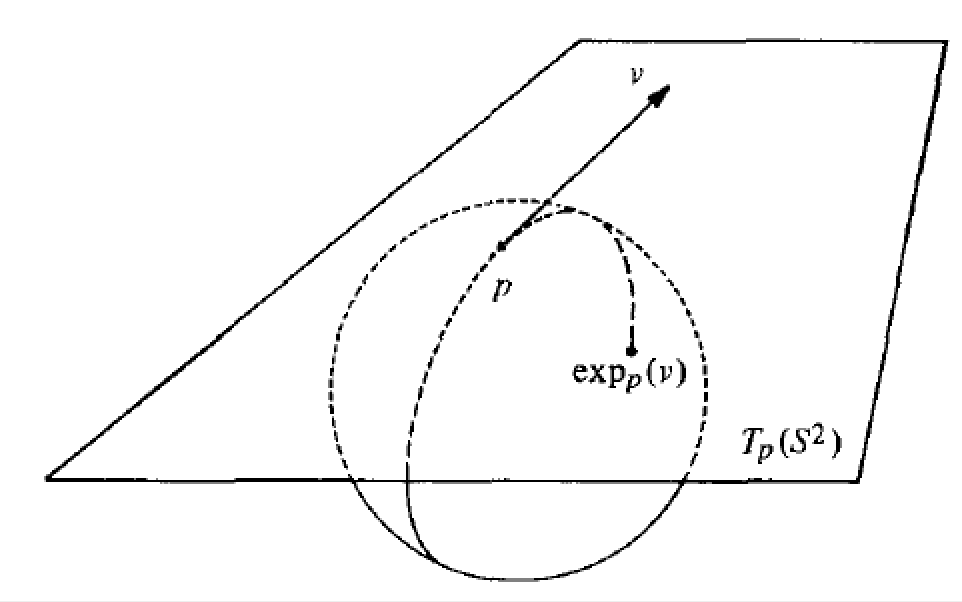
\includegraphics[scale = 0.43]{exp_map.png}}
\end{minipage}
\caption{\scriptsize
\textbf{The exponential map $\exp_{p}(\mb{v})$ is the point at $\cS$ obtained by laying off a length equal to $\norm{\mb{v}}{}$ along the geodesic that passes through $p$ in the direction of $\mb{v}$.  }}
\end{figure} 

\item Its \textbf{geometric interpretation} is given as laying off a length equal to $\norm{\mb{v}}{}$ along the geodesic that passes through $p$ in the direction of $\mb{v}$; then \textbf{point} of $\cS$ thus \textbf{obtained} is denoted by $\exp_{p}\paren{\mb{v}}$. 


\item The \emph{\textbf{appropriateness}} of the definition of the exponential map relies on the \textbf{\emph{uniqueness}} of the ordinary differential equations that define the geodesic with initial value $\gamma(0)$ and $\lambda\,\dot{\gamma}(0)$ for $t$ sufficiently small. Then for the tangent vector $\mb{v}$ small enough, there exists a geodesic at $p'= \gamma(t,\mb{v})$ with $t$ small such that $\gamma(0)$ and $\lambda\,\dot{\gamma}(0)$.

\item  \begin{proposition}\label{prop: exp_map_diff}
Given $p\in \cS$, there exists an $\epsilon>0$ such that $\exp_{p}$ is defined and \textbf{differentiable} in the interior $B_{\epsilon}$ of a disk of radius $\epsilon$ of $T_{p}S$, with the center at origin. 
\end{proposition}

\item  \begin{proposition}\label{prop: exp_map_diffeomorph}
The exponential map $\exp_{p}: B_{\epsilon}\subset T_{p}\cS \rightarrow \cS$ is a \textbf{diffeomorphism} in a neighborhood $U\subset B_{\epsilon}$ of the origin $0$ of $T_{p}\cS$. 
\end{proposition}
\begin{proof}
We shall show that $d(\exp_{p})$ is nonsingular at $0\in T_{p}\cS$. To do this, we identify the space of tangent vectors of $T_{p}\cS$ at $0$ with $T_{p}\cS$ itself. Consider the curve $\alpha(t) = t\mb{v}, \mb{v}\in T_{p}\cS$. It is clear that $\alpha(0) = 0$ and $\dot{\alpha}(0) = \mb{v}$. The curve $\exp_{p}\circ \alpha (t) = \exp_{p}\paren{t\mb{v}}$ has at $t=0$ the tangent vector 
\begin{align*}
\rlat{\frac{d}{dt}\paren{\exp_{p}\paren{t\mb{v}}}}{t=0} &= \rlat{\frac{d}{dt}\paren{\gamma\paren{t, \mb{v}}}}{t=0} = \mb{v}.
\end{align*}
It follows that 
\begin{align*}
\paren{d\exp_{p}}_{0}(\mb{v}) &= \mb{v},
\end{align*}
which shows that $d\exp_{p}$ is nonsingular at $t=0$. By applying the inverse function theorem, we complete the proof of the proposition. \QEDA 
\end{proof}
\end{itemize}

\subsection{Geodesic Polar Coordination}
\begin{itemize}
\item The \emph{\textbf{image}} of \emph{the exponential map} $V = \exp_{p}(U) \subset \cS$ of a neighborhood $U$ of the origin of $T_{p}\cS$ restricted to which $\exp_{p}$ is a \emph{\textbf{diffeomorphism}} is called a \emph{\textbf{normal neighborhood}} of $p\in \cS$.

\begin{figure}[htb]
\centering
\begin{minipage}{0.6\linewidth}
 \centerline{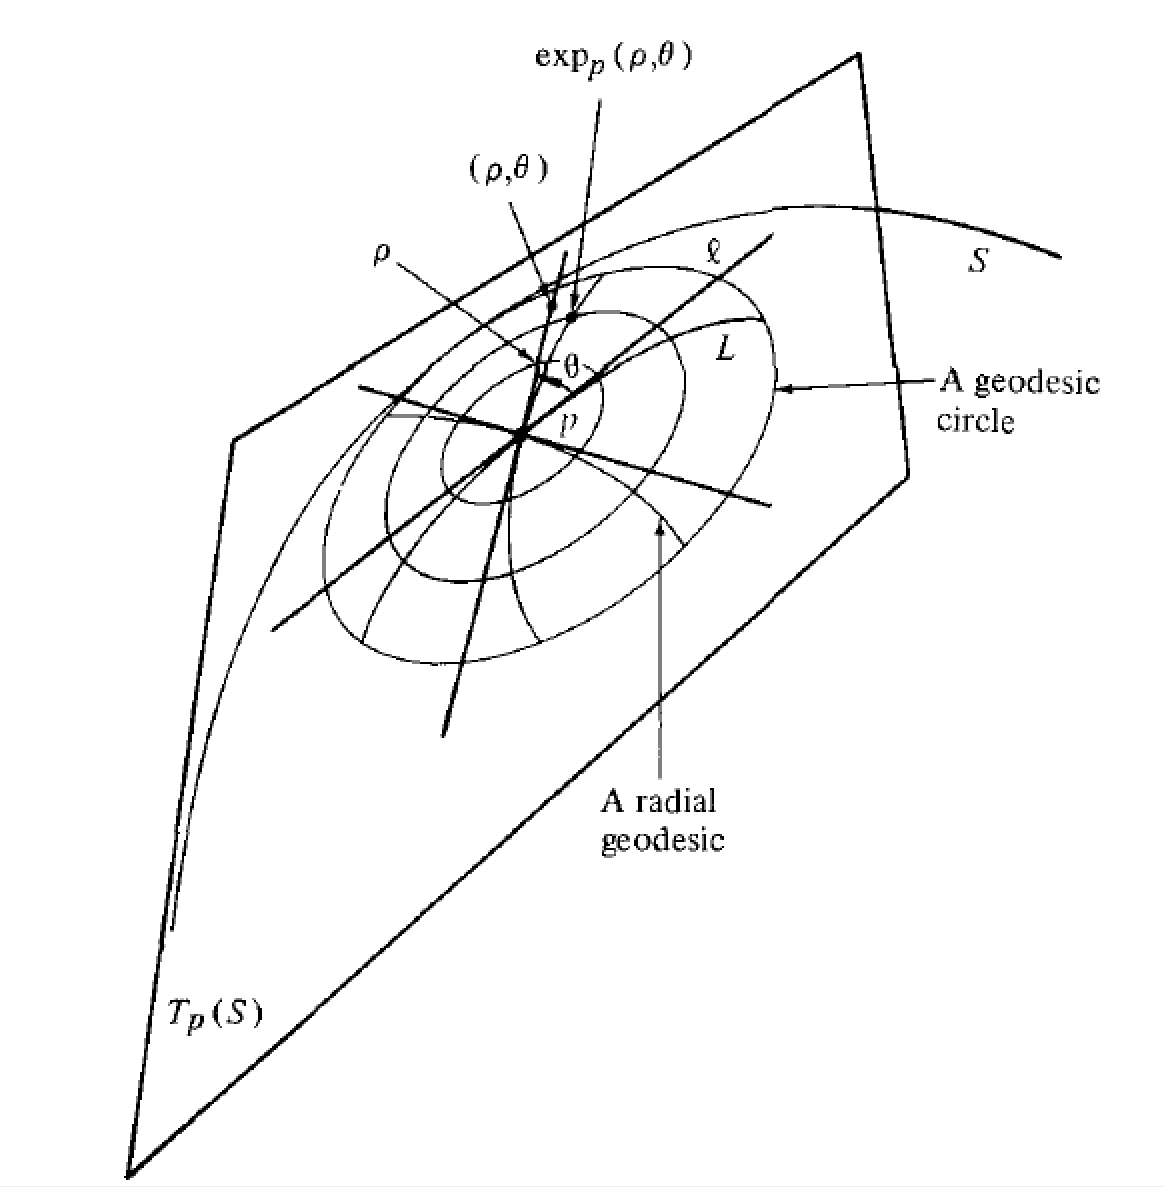
\includegraphics[scale = 0.43]{geo_polar_coord.png}}
\end{minipage}
\caption{\scriptsize
\textbf{The geodesic polar coordinate system is defined in the image of exponential map restricted to which the exponential map is a diffeomorphism.  Observe that the polar coordinate in the plane are not defined in the closed half line $\ell$ which corresponds to $\theta=0$. }}
\label{fig: geo_polar_coord}
\end{figure}

\item Since the \emph{exponential map} at $p \in \cS$ is a \emph{diffeomorphism} on $U$, it may be used to introduce \emph{\textbf{coordinates}} in $V$. Among the coordinate systems thus introduced, the most usual are:
\begin{enumerate}
\item The \emph{\textbf{normal coordinates}} which correspond to a system of \emph{rectangular} coordinates in the tangent plane $T_{p}\cS$.

The normal coordinates are obtained by choosing in the plane $T_{p}\cS$, $p \in \cS$, two \textbf{orthogonal unit vectors} $\mb{e}_1$ and $\mb{e}_2$. Since $\exp_{p}: U \rightarrow V \subset \cS$ is a \emph{diffeomorphism}, it satisfies the conditions for a parametrization in $p$. If $q \in V$,then $q = \exp_{p}(\mb{w})$, where $\mb{w} = u \mb{e}_1+ v \mb{e}_2 \in U$, and we say that $q$ has coordinates $(u, v)$. It is clear that the normal coordinates thus obtained depend on the \emph{\textbf{choice of basis vector}} $\mb{e}_1$ and $\mb{e}_2$.


\item The \emph{\textbf{geodesic polar coordinates}} which correspond to \emph{\textbf{polar coordinates}} in the tangent plane $T_{p}\cS$ (Fig. \ref{fig: geo_polar_coord}).

In particular, choose in the tangent plane $T_{p}\cS, p\in \cS$, a system of \emph{\textbf{polar coordinates}} $(\rho, \theta)$, where $\rho$ is the \emph{polar radius} and $\theta, \; 0<\theta<2\pi$, is the \emph{polar angle}, the \textbf{\emph{pole}} of which is the origin $0$ of $T_{p}\cS$. The point on $\cS$ is given by $\exp_{p}(\rho, \theta).$ Observe that the polar coordinate in the plane are not defined in the closed half line $\ell$ which corresponds to $\theta=0$. Set $\exp_{p}(\ell) = L$. Since $\exp_{p}: (U \setminus \set{\ell})\; \rightarrow (V \setminus \set{L})$ is still a diffeomorphism, we may parameterize the points of $(V \setminus \set{L})$ by the coordinates $(\rho, \theta)$, which are called \emph{\textbf{geodesic polar coordinate system}}. 

The \emph{image} of $\exp_{p}: U\rightarrow V$ of circles in $U$, centered at $0$ is called \emph{\textbf{geodesic circles}} of $V$ and the \emph{image} of $\exp_{p}$ of lines through $0$ will be called \emph{\textbf{radical geodesics}} of $V$. In $(V \setminus \set{L})$, these are curves $\rho = const.$ and $\theta = const.$, respectively. 
\end{enumerate}

\item We compare two different coordinates for the coefficients of first fundamental form
\begin{itemize}
\item In a system of \emph{\textbf{normal coordinates}} centered in $p$, the geodesics that pass through $p$ are the images by $\exp_{p}$ of the lines $u = a\,t$, $v = b\,t$ which pass through the origin of $T_{p}\cS$. Observe also that at $p$ the \emph{\textbf{coefficients of the first fundamental form}} in such a system are given by $E(p) = G(p) = 1$, $F(p) = 0$.

\item As for the geodesic polar coordinates, we have the following proposition.
\end{itemize}

\item \begin{proposition}\label{prop: exp_map_first_fund}
Let $\mb{x}: (U \setminus \set{\ell})\rightarrow (V \setminus \set{L})$  be a system of \textbf{geodesic polar coordinates} $(\rho, \theta)$. Then the coefficients $E\equiv E(\rho, \theta)$, $F\equiv F(\rho, \theta)$ and $G\equiv G(\rho, \theta)$ of the first fundamental form satisfies the conditions
\begin{align*}
E = 1, \quad F=0, \quad \lim_{\rho \rightarrow 0}G = 0, \quad \lim_{\rho\rightarrow 0}(\sqrt{G})_{\rho} = 1.
\end{align*}
\end{proposition}
\begin{proof}
By definition of exponential map, $\rho$ measures the arc length along the curve $\theta = const.$ It follows immediately that $E= 1$ (the length of $(d/dt)\gamma(t,(1,\theta_{0}))$ is one by definition). 

From differential equation of the geodesic, $\theta = const.$ is a geodesic, we conclude that $\Gamma_{11}^{2} = 0$. Also from the equation for Christoffel symbol, we have that
\begin{align*}
0= \frac{1}{2}E_{\rho}&= \Gamma_{11}^{1}E = \Gamma_{11}^{1}.
\end{align*}
Also using the relation of Christoffel symbols, $F_{\rho} = 0$ and therefore $F(\rho, \theta)$ does not depend on $\rho$.

For each $q\in V$, denote the curve $\alpha(\sigma)$ as the geodesic circle that passes through $q$, where $\sigma\in [0,2\pi]$. We shall denote by $\gamma(s)$, where $s$ is the arc length of $\gamma$, the radical geodesic that pass through $q$.  With this notation, we write
\begin{align*}
F(\rho, \theta) &= \inn{\frac{d\alpha}{d\sigma}}{\frac{d\gamma}{ds}}.
\end{align*}
The coefficient $F$ does not depend on $\rho$. However, if the radical geodesic $\theta = const.$, the second member of the above equation is defined for every point of this geodesic. Since at $p$, $\alpha(\sigma) = p$ for all $\sigma$, that is $\frac{d\alpha}{d\sigma} = 0$, we obtain
\begin{align*}
\lim_{\rho \rightarrow 0}F(\rho, \theta) &= \lim_{\rho \rightarrow 0}\inn{\frac{d\alpha}{d\sigma}}{\frac{d\gamma}{ds}} = 0
\end{align*}
Together with $F$ does not depend on $\rho$, thus $F = 0$.

To show the last assertion, we choose a system of normal coordinate $(\bar{u}, \bar{v})$ in $p$ such that the change of coordinate is given as 
\begin{align*}
\bar{u} = \rho\cos\theta; && \bar{v} = \rho\sin\theta, && \rho\neq 0, \; 0< \theta<2\pi.
\end{align*}
By recalling that 
\begin{align*}
\sqrt{EG- F^{2}} &= \sqrt{\bar{E}\bar{G} - \bar{F}^{2}}\;\frac{\partial (\bar{u}, \bar{v})}{\partial (\rho,\theta)}
\end{align*}
where $\frac{\partial (\bar{u}, \bar{v})}{\partial (\rho,\theta)} = \rho$ is the Jacobian of the change of the coordinates and $\bar{E},\bar{G}, \bar{F}$ are coefficients of the first fundamental form in $(\bar{u}, \bar{v})$, we have
\begin{align*}
\sqrt{G} &= \rho \sqrt{\bar{E}\bar{G} - \bar{F}^{2}}, \quad \rho \neq 0.
\end{align*}
Since at $p$, $\bar{E}=\bar{G}=1, \bar{F}=0$ (as it is the orthonormal coordinates in $p$), we conclude that 
\begin{align*}
\lim_{\rho \rightarrow 0}\sqrt{G} =0 && \lim_{\rho \rightarrow 0}(\sqrt{G})_{\rho} = 1,
\end{align*} 
which concludes the proof of the proposition.\QEDA
\end{proof}

\item The geometric meaning of the fact that $F=0$  is that in a normal neighborhood \emph{\textbf{the family of geodesic circles} are \textbf{orthogonal} to \textbf{the family of radical geodesics}}. This fact is known as \emph{\textbf{Gauss Lemma}}. 

\item Consider the \textbf{\emph{Gaussian curvature}} $\mb{K}$ in a \textbf{\emph{polar system}}. Since $E=1,F=0$, it means that 
\begin{align}
\mb{K} &= -\frac{(\sqrt{G})_{\rho\rho}}{\sqrt{G}} \label{eqn: Gauss_Jacobi_formula}
\end{align}
In other words, this is the differential equation for $\sqrt{G}(\rho, \theta)$ given the curvature $\mb{K}(\rho, \theta)$.  
\begin{align}
(\sqrt{G})_{\rho\rho} + \mb{K}\sqrt{G} = 0 \label{eqn: Gauss_Jacobi_formula2}
\end{align} The equation \eqref{eqn: Gauss_Jacobi_formula2} (or \eqref{eqn: Gauss_Jacobi_formula}) is called the \emph{\textbf{Gauss-Jacobi equation}}. 

For constant $\mb{K}$, the equation \eqref{eqn: Gauss_Jacobi_formula} is a linear differential equation of the second order with constant coefficients. 


\item \begin{theorem}\label{thm: minding_thm} (\textbf{Minding}). \citep{do1976differential} \\
Any two regular surfaces with the \textbf{same constant Gaussian curvature} are \textbf{locally isometric}. More precisely, let $\cS_{1}$ and $\cS_{2}$ be two regular surfaces with the same constant curvature $\mb{K}$. Choose points $p_{1}\in \cS_{1}$, $p_{2}\in \cS_{2}$, and orthonormal basis $\set{\mb{e}_{1}, \mb{e}_{2}}\in T_{p_{1}}\cS_{1}$ and $\set{\mb{f}_{1}, \mb{f}_{2}}\in T_{p_{2}}\cS_{2}$. Then there exists neighborhood $V_{1}$ of $p_{1}$, $V_{2}$ of $p_{2}$ and an \textbf{isometry} $\psi: V_{1}\rightarrow V_{2}$ such that $d\psi(\mb{e}_{1}) = \mb{f}_{1} $ and  $d\psi(\mb{e}_{2}) = \mb{f}_{2} $.
\end{theorem}

\begin{figure}[tbh]
\centering
\begin{minipage}{0.6\linewidth}
 \centerline{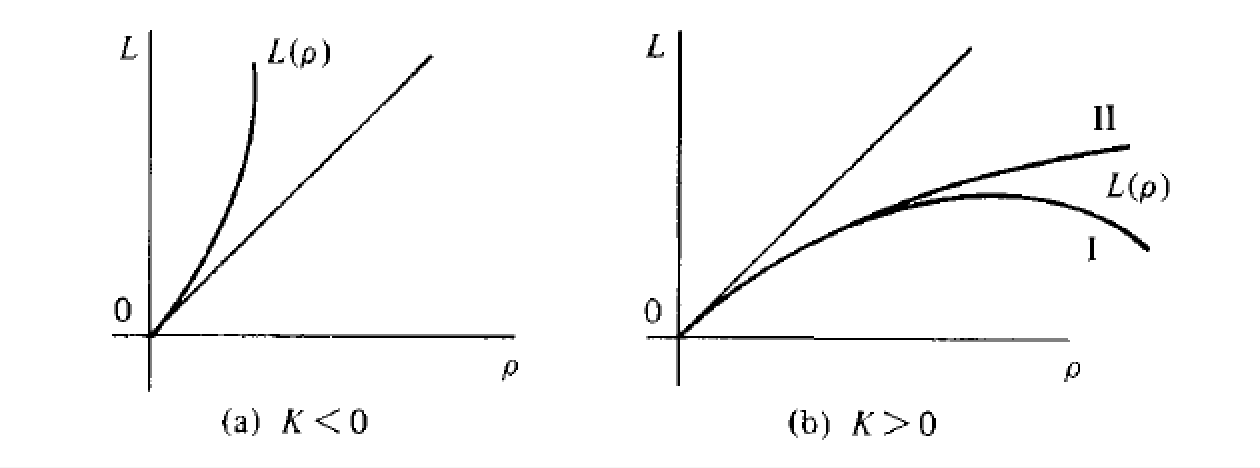
\includegraphics[scale = 0.43]{arc_length_geodesic.png}}
\end{minipage}\\
\begin{minipage}{0.6\linewidth}
 \centerline{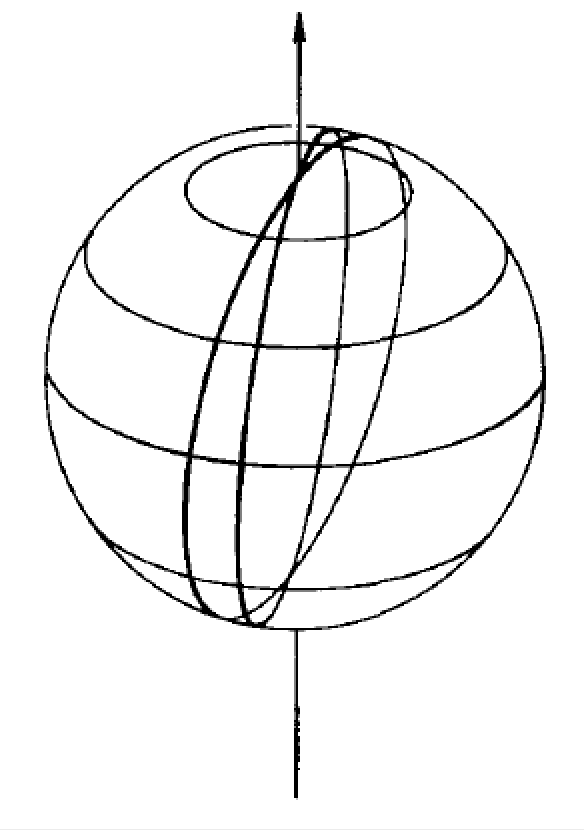
\includegraphics[scale = 0.43]{arc_length_geodesic2.png}}
\end{minipage}
\caption{\scriptsize
\textbf{The arc length of the geodesic joins two radical geodesics $\theta_{0}$ and $\theta_{1}$. For hyperbolic surface (a), the two radical geodesics will get farther apart as they depart from the origin. For the elliptic surface (b), these two geodesic may come closer after a certain point. Like in the sphere, two geodics become closer after passing the equator. }}
\label{fig: arc_length_geo}
\end{figure}

\item In the case that $\mb{K}$ is not constant but maintains its sign, the expression $\mb{K}\sqrt{G}=-(\sqrt{G})_{\rho\rho}$ has a nice intuitive meaning.

Consider the arc length $L(\rho)$ of the curve $\rho = const.$ between two close geodesics $\theta_{0}$ and $\theta_{1}$: 
\begin{align*}
L(\rho) &= \int_{\theta_{0}}^{\theta_{1}}\sqrt{G(\theta, \rho)}d\theta.
\end{align*}

\begin{enumerate}
\item Assume that $\mb{K}<0$ (\emph{\textbf{hyperbolic geometry}}), since $\lim_{\rho\rightarrow 0}(\sqrt{G})_{\rho} = 1$, $\mb{K}\sqrt{G} = -(\sqrt{G})_{\rho\rho}$, the function $L(\rho)$ \emph{\textbf{increases}} as $\rho$ \emph{\textbf{increase}}, the \emph{\textbf{geodesics} $\theta_{0}$ and $\theta_{1}$ are getting farther and farther \underline{\textbf{apart} from each other}}.  Figure \ref{fig: arc_length_geo} (top left).

\item On the other hand, when $\mb{K}>0$ (\emph{\textbf{elliptic geometry}}), the geodesics $\theta_{0}$ and $\theta_{1}$ \emph{\textbf{may or may not \underline{come closer}}} to each other after a certain value of $p$, and this depends on the \emph{\textbf{Gaussian curvature}}. See Figure \ref{fig: arc_length_geo} (top right).
\end{enumerate}


\item As a last application of the geodesic polar coordinates, we shall study some minimal properties of geodesics. \emph{\textbf{A fundamental property} of a geodesic is the fact that, \textbf{locally}, it \textbf{minimizes arc length}}. 

\begin{proposition}\label{prop: geo_minimal_arc}
(\textbf{The geodesic joins two points has the minimal arc length}).\\ 
Let $p$ be a point on a surface $\cS$. Then there exists a neighborhood $W\subset \cS$ of $p$ such that if $\gamma: I\rightarrow W$ is  a parameterized \textbf{geodesic} with $\gamma(0) = p$, $\gamma(t_{1}) = q,\; t_{1}\in I$, and $\alpha: [0,t_{1}]\rightarrow \cS$ is a parameterized regular curve joining $p$ and $q$, we have
\begin{align*}
\ell_{\gamma} \le \ell_{\alpha},
\end{align*}
where $\ell_{\alpha}$ denotes the arc length of the curve $\alpha$. Moreover, if $\ell_{\gamma} = \ell_{\alpha}$, then the trace of $\gamma$ \textbf{coincides} with the trace of $\alpha$ between $p$ and $q$.
\end{proposition}
Note the above proposition holds only \emph{\textbf{locally}}. It is seen that two nonantipodal points of a sphere may be connected by two meridians of unequal lengths, and only the smallest one satisfies the property. That is, the geodesics, if sufficiently extended, may not be the shortest path between its end points. 

\item \begin{proposition}\label{prop: regular_minimal_arc}
(\textbf{The minimal arc length regular curve joins two points is the geodesic}).\\ 
Let $\alpha: [0,t_{1}]\rightarrow \cS$ is a parameterized regular curve with parameter as the arc length. Suppose that the arc length of $\alpha$ between any two points $t, \tau \in I$ is \textbf{smaller than or equal to} the arc length of any regular parameterized curve joining $\alpha(t), \alpha(\tau)$. Then $\alpha$ is a \textbf{geodesic}. 
\end{proposition}
\end{itemize}

\newpage
\section{Homework and Examples}
\begin{enumerate}
\item  \begin{example} \citep{do1976differential} (p260. 1.)
\begin{enumerate}
\item Show that if a curve $\cC \subset \cS$ is both a line of curvature and a geodesic, then the curve $\cC$ is a plane curve, i.e. its torsion is zero $\mb{t} = 0$.

\item Show that if a (nonrectilinear) geodesic is a plane curve, then it is a line of curvature.

\item Give an example of a line of curvature which is a plane curve and not a geodesic. 
\end{enumerate}
\end{example}

\item \begin{example} \citep{do1976differential} (p261. 8.)\\
Show that if all the geodesic of a connected surface are plane curves, then the surface is contained in a plane or a sphere. 
\end{example}


\item \begin{example}\citep{do1976differential} (p439.)
(\textbf{The tangent bundle as a smooth manifold of dimension} $2n$) \\
Consider the surface in $\mb{R}^{3}$ with parameterization $\mb{x}: U \subset \bR^{2}\rightarrow \cS$. The set $T\cS \equiv \set{(p, \mb{v}): \mb{v}\in T_{p}\cS}$ where $T_{p}\cS$ is the tangent space at $p$ is called the \emph{tangent bundle}.  

The tangent bundle equips with a natural parameterization  $\mb{y}: U \times \bR^{2} \rightarrow T\cS$ by 
\begin{align*}
\mb{y}(u, v, w', z') &= \paren{\mb{x}(u,v),  w'\mb{x}_{u} + z'\mb{x}_{v}}  = \paren{p, \mb{v}},\quad (w',z')\in \bR^{2}
\end{align*} 
where $(u,v)$ is the coordinate of $p$ in $\cS$ and $(w',v')$ is the coordinate of $\mb{v}$ in $T_{p}\cS$.  

We can check the pair $\paren{ U \times \bR^{2},  \mb{y}}$ is a differentiable structure for $T\cS$. Note that $d\mb{x}_{q}(\bR^{2}) = T_{\mb{x}(q)}\cS, q\in U$. If $(p, \mb{v}) \in \mb{y}_{a}(U_{a}\times \bR^{2}) \cap \mb{y}_{b}(U_{b}\times \bR^{2}) $, then
\begin{align*}
\bigcup_{a}\mb{y}_{a}(U_{a}\times \bR^{2}) = T\cS
\end{align*}
since $\bigcup_{a}\mb{x}_{a}(U_{a}) = \cS$ and $(d\mb{x}_{a})_{q}(\bR^{2}) = T_{\mb{x}(q)}\cS, q\in U$.
Also, when
\begin{align*}
(p, \mb{v})  &= (\mb{x}_{a}(q_{a}),  d\mb{x}_{a}(\mb{w}_{a})) = (y_{b}(q_{b}), d\mb{x}_{b}(\mb{w}_{b}))
\end{align*}
where $q_{a}\in U_{a}$ and $q_{b}\in U_{b}$, $\mb{w}_{a}, \mb{w}_{b}\in \bR^{2}$,  
\begin{align*}
\mb{y}_{b}^{-1}\circ \mb{y}_{a}(q_{a}, \mb{w}_{a}) &= \mb{y}_{b}^{-1}\paren{\mb{x}_{a}(q_{a}),  d\mb{x}_{a}(\mb{w}_{a})}\\
&= \paren{ \mb{x}_{b}^{-1}\circ\mb{x}_{a}(q_{a}), d(\mb{x}_{b}^{-1}\circ \mb{x}_{a})(\mb{w}_{a})  }.
\end{align*}
Since $(\mb{x}_{b}^{-1}\circ\mb{x}_{a})$ is differentiable, so is $d(\mb{x}_{b}^{-1}\circ\mb{x}_{a})$. It follows that $\mb{y}_{b}^{-1}\circ \mb{y}_{a}$ is differentiable. 

The tangent bundle is a natural space to be considered by dealing with second-order ordinary differential equations (e.g. in describing the geodesic on $\cS$ ) 
\begin{align*}
\frac{d^{2}u}{dt^{2}} &= f_{1}\paren{u, v, \frac{du}{dt}, \frac{dv}{dt}}\\
\frac{d^{2}v}{dt^{2}} &= f_{2}\paren{u, v, \frac{du}{dt}, \frac{dv}{dt}}.
\end{align*}
By introducing $\frac{du}{dt} = w'$ and $\frac{dv}{dt} = z'$,  it becomes a system of first-order differential equations
\begin{align*}
\frac{du}{dt} &= w'\\
\frac{dv}{dt} &= z'\\
\frac{dw'}{dt} &= f_{1}\paren{u, v, w', z'}\\
\frac{dz'}{dt} &= f_{2}\paren{u, v, w', z'}
\end{align*}
and the solution is the trajectory of vector field $(u, v, w', v')$ given locally in the tangent bundle $T\cS$. It can be shown that such a vector field is well-defined in $T\cS$; that is, in the intersection of two coordinate neighborhoods, the vector fields in above equations agree. 

This field or trajectory $(u(t), v(t), w'(t), v'(t))$ is called the \emph{geodesic flow} on $T\cS$. It is a natural object to study global properties of the geodesic on $\cS$.
\end{example}


\item  \begin{example} \citep{do1976differential} (p296. 12.)\\
A diffeomorphism $\varphi: \cS_{1} \rightarrow \cS_{2}$ is said to be a \emph{geodesic mapping} if for every geodesic $\cC\subset \cS_{1}$ of $\cS_{1}$, the regular curve $\varphi\paren{\cC} \subset \cS_{2}$ is a geodesic of $\cS_{2}$. If $U$ is a neighborhood of $p\in \cS_{1}$, then $\varphi: U \rightarrow \cS_{2}$ is said to be a \emph{local geodesic mapping} in $p$ if there exists a neighborhood $V$ of $\varphi(p)$ in $\cS_{2}$ such that $\varphi: U\rightarrow V$ is a geodesic mapping. 
\begin{enumerate}
\item Show that if $\varphi: \cS_{1} \rightarrow \cS_{2}$ is both a geodesic mapping and a conformal mapping, then $\varphi$ is a \emph{similarity};  that is,
\begin{align*}
\inn{\mb{v}}{\mb{u}} &= \lambda\inn{d\varphi_{p}(\mb{v})}{d\varphi_{p}(\mb{w})}, \quad p\in \cS_{1}, \mb{v},\mb{w} \in T_{p}\cS_{1},
\end{align*}
where $\lambda$ is constant.  

\item Let $\bS^{2} = \set{(x,y,z) \in \bR^{3}; x^{2}+ y^{2}+ z^{2} = 1}$ be the unit sphere, $\bS^{-} = \set{(x,y,z) \in \bS^{2}; z < 0}$ be the lower hemisphere, and $P$ be the plane $z=-1$. Prove that the map (central projection) $\varphi: \bS^{-} \rightarrow P$ which takes a point $p\in \bS^{-}$ to the intersection of $P$ with the line that connects $p$ to the center of $\bS^{2}$ is a geodesic mapping. 

\item Show that a surface of constant curvature admits a local geodesic mapping into the plane for every $p\in \cS$.
\end{enumerate}
\end{example}

\item \begin{example}\citep{do1976differential} (p307. 4.)\\
The \emph{energy} $E$ of a curve $\alpha: [a,b] \rightarrow \cS$ is defined by 
\begin{align*}
E(\alpha) &= \int_{a}^{b}\abs{\dot{\alpha}(t)}^{2}dt.
\end{align*}
\begin{enumerate}
\item Show that $\paren{\ell(\alpha)}^{2} \le (b-a)E(\alpha)$ and that the equality holds if and only if $t$ is proportional to the arc length. 

\item Conclude from the above that if $\gamma: [a,b]\rightarrow \cS$ is a minimal geodesic with $\gamma(a) = p$, $\gamma(b) = q$, then for any curve $\alpha:  [a,b]\rightarrow \cS$, joining $p$ and $q$, we have $E(\gamma) \le E(\alpha) $ with the equality holds if and only if $\alpha$ is a minimal geodesic. 
\end{enumerate}
\end{example}

\item \begin{example}\citep{do1976differential} (p306. 3.)\\
Let $\alpha: I=[0,l]\rightarrow \cS$ be a simple, parameterized, regular curve. Consider a unit vector field $\mb{v}(t)$ along $\alpha$, with $\inn{\dot{\alpha}(t)}{\mb{v}(t)}=0$ and a mapping $\mb{x}: \bR\times I \rightarrow \cS$ given by 
\begin{align*}
\mb{x}(s,t) &= \exp_{\alpha(t)}\paren{s\mb{v}(t)}, \quad s\in \bR;\; t\in I.
\end{align*}
\begin{enumerate}
\item Show that $\mb{x}$ is differentiable in the neighborhood of $I$ in $\bR\times I$ and that $d\mb{x}$ is nonsingular in $(0,t),\;t\in I$.
\item Show that there exits $\epsilon>0$ such that $\mb{x}$ is one-to-one in the rectangle $t\in I$, $\abs{s}<\epsilon$.
\item Show that in the open set $t\in (0,l), \abs{s}<\epsilon$, $\mb{x}$ is parameterization of $\cS$, the coordinate neighborhood of which contains $\alpha((0,l))$. The coordinates thus obtained are called \emph{geodesic coordinate} (or, \emph{Fermi's coordinate}) of basis $\alpha$. Show that in such a system $F=0, E=1$. Moreover, if $\alpha$ is a geodesic parameterized by the arc length,  $G(0,t) = 1$ and $G_{s}(0,t) = 0$.
\item Establish the following analogue of the Gauss lemma. Let $\alpha: I\rightarrow \cS$ be a regularized parameterized curve and let $\gamma_{t}(s),\;t\in I$ be a family of geodesics parameterized by arc length $s$ and given by $\gamma_{t}(0)=\alpha(t), \set{\dot{\gamma}_{t}(0), \dot{\alpha}_{t}}$ is a positive orthogonal basis. Then, for a fixed $\bar{s}$, sufficiently small, the curve $t\rightarrow \gamma_{t}(\bar{s}), t\in I$, intersects all $\gamma$, orthogonally (such curves are called \emph{geodesic parallels}. )
\end{enumerate}
\end{example}

\item \begin{example}
Define \emph{the derivative $\mb{w}(f)$ of a differentiable function $f: U\subset \cS \rightarrow \bR$ relative to a vector field} $\mb{w}$ in $U$ by 
\begin{align*}
\mb{w}(f)(q) &= \rlat{\frac{d}{dt}\paren{f\circ \alpha}}{t=0},\quad q\in U
\end{align*}
where $\alpha: I\rightarrow \cS$ is the trajectory of $\mb{w}$ passing through $q$ such that $\alpha(0) = q, \alpha'(0)=\mb{w}(q)$. Prove that 
\begin{enumerate}
\item $\mb{w}$ is differentiable in $U$ if and only if $\mb{w}(f)$ is differentiable for all differentiable function $f$ in $U$.
\item Let $\lambda, \mu\in \bR$ and $g: U\subset \cS \rightarrow \bR$ be a differentiable function on $U$ then 
\begin{align*}
\mb{w}\paren{\lambda\,f+ \mu\, g} &= \lambda\,\mb{w}(f) + \mu\,\mb{w}(g),\\
\mb{w}\paren{fg} &= \mb{w}(f)g +f\mb{w}(g).
\end{align*}
\end{enumerate}
\end{example}
Note that if $\mb{w} = \partdiff{}{u}$, then $\paren{\partdiff{}{u}}(f)(q) = \partdiff{f}{u}(q)$, which justify the notion.

\begin{solution}
\begin{enumerate}
\item We note that for $\mb{w}(u,v) = a(u,v)\partdiff{}{u}+ b(u,v)\partdiff{}{v}$
\begin{align*}
\mb{w}(f)(q) &= \rlat{\frac{d}{dt}\paren{f\circ \alpha}}{t=0},\\
&= \rlat{a(u,v)\partdiff{f}{u}}{q} + \rlat{b(u,v)\partdiff{f}{v}}{q} 
\end{align*}
Thus we consider the vector field $\mb{w}: \mathcal{C}^{\infty}(U) \rightarrow \mathcal{C}^{\infty}(U) $ as a mapping on $f$.
\begin{align*}
d(\mb{w}(f))(q) &= \partdiff{a(u,v)}{u}\partdiff{f}{u}+ a(u,v)\partdiff{^{2}f}{u^{2}}+ \partdiff{b(u,v)}{u}\partdiff{f}{v}+ b(u,v)\partdiff{^{2}f}{u\partial v}\\
&+\partdiff{a(u,v)}{v}\partdiff{f}{u}+ a(u,v)\partdiff{^{2}f}{u\partial v}+ \partdiff{b(u,v)}{v}\partdiff{f}{v}+ b(u,v)\partdiff{^{2}f}{v^{2}}\\
&= (d\mb{w})(f)(q) + \mb{w}(df)(q)
\end{align*}




$\Rightarrow$ Given that $\mb{w}$ is differentiable, i.e. $a(u,v), b(u,v)$ is differentiable, it is clear by the chain rule that for every $f$ differentiable, then  the RHS exists, thus
i.e. $\mb{w}(f)$ is differentiable.

$\Leftarrow$  Given that $\mb{w}(f)$ is differentiable for all $f \in \mathcal{C}^{\infty}(U)$, then we choose $f_{i}$ as all the first integral of $\mb{w}$ restricted in each axis,  
since $0= d(\mb{w}(f)) = (d\mb{w})(f)+ \mb{w}(df)$, we see that there exists $n$ independent equations, 
\begin{align*}
(d\mb{w})(f_{i}) &= -\mb{w}(df_{i}) \quad i=1,\ldots,n
\end{align*}
for all $f\in \mathcal{C}^{\infty}(U)$. Thus the differential $d\mb{w}$ exists as $\mb{w}(df)\neq 0$. 

\end{enumerate}
\end{solution}
\end{enumerate}
\newpage
\bibliographystyle{plainnat}
\bibliography{book_reference.bib}
\end{document}